\chapter{EG-CNTFET as sensor}
\label{cap:chapter4}

\newpage
\thispagestyle{empty}
\ % Empty page
\newpage

%%%%%%%%%%%%%%%%%%%%%%%%%%%%%%%%%%%%%%%%%%%%%%%%%%%%%%%%%%%%%%%%%%%%%%

\section{EG-CNTFET functionalization}
\label{sec:EGFETfunctionalization}

%% originally in chapter 2
% One of the most common approaches involves attaching the recognition element to the semiconductor itself, either through covalent or non-covalent methods. Non-covalent functionalization involves weak interactions, \ce{\pi-\pi} stacking, hydrophobic or van der Waals forces: in these cases, the recognition elements are adsorbed on the surface of the semiconductor without interfering with the molecular structure.
% Covalent functionalization, on the other hand, involves sharing of electrons between atoms of the recognition element and the semiconductor.

% chemically bonds functional groups (\eg{} carboxyl, amine, thiol) to the CNT surface, enabling strong and stable attachment of bio-molecules. Typically, oxygen-containing groups are introduced using strong oxidizing agents, followed by activation with carbodiimide chemistry (EDC/NHS) to facilitate binding. While covalent attachment ensures stability, it can introduce defects in the CNT structure, potentially altering its electronic properties. To mitigate this, an alternative approach involves using binding molecules (\eg{} PBASE, diazonium salts) that attach non-covalently to CNTs while providing functional groups for covalent linkage with bio-recognition elements.

% Another strategy is functionalizing the gate electrode, which allows biomolecule attachment without disrupting CNT conductivity. For gold gate electrodes, thiol chemistry is commonly employed, where self-assembled monolayers of alkanethiols enable bio-recognition elements to bind via carboxyl or amine groups. For example, 3-mercaptopropionic acid (MPA) can link bio-molecules to gold surfaces while preserving the sensor's electrical properties.

% A more recent approach involves modifying the substrate beneath the CNTs. In this method, molecules like glutaric acid create a binding layer between the substrate and the bio-recognition element. This technique preserves the CNTs' electrical and structural integrity while enabling efficient functionalization.

% Each of these strategies offers distinct advantages, with the choice depending on the required stability, electronic performance, and specificity of the sensor.

% \note{The most common approach is the functionalization of the semiconducting CNT channel, which can be achieved through covalent or non-covalent modifications. Non-covalent functionalization relies on physical adsorption via π–π interactions, hydrophobic forces, or electrostatic attraction, preserving the CNTs' electronic properties. In contrast, covalent functionalization involves chemically attaching functional groups (e.g., carboxyl, amine, or thiol) that react with biomolecules, often using strong oxidizing agents like sulfuric acid and hydrogen peroxide. While this method provides strong and stable bonding, it may introduce defects that alter the CNTs' electrical behavior. Alternatively, an indirect approach uses linker molecules, such as PBASE or diazonium salts, which facilitate biomolecule attachment while preserving the CNT structure.
% %
% Another strategy involves functionalizing the gate electrode, particularly in devices with gold gates, where thiol-based self-assembled monolayers (SAMs) enable stable attachment of biomolecules. For instance, 3-mercaptopropionic acid (MPA) can be used to bind biomolecules via thiol–gold interactions while maintaining available functional groups for further coupling.
% %
% A more recent approach focuses on substrate functionalization, modifying the surface beneath the CNTs rather than the nanotubes themselves. This method, demonstrated by Joshi et al., involves using glutaric acid as a linker, binding to the substrate while leaving functional groups available for biomolecule attachment. A key advantage of this technique is that it preserves the structural and electrical properties of the CNTs while enabling functionalization.
% %
% Each of these strategies offers unique benefits, with the choice depending on the desired sensor properties and functionalization stability.}

% \AT{Previous projects in our laboratory have employed the first strategy for device functionalization, specifically targeting the semiconducting channel. One notable example is the use of an ionophore-containing membrane for ammonium ion detection. In this case, there was no chemical interaction between the membrane and the carbon nanotubes (CNTs); instead, the membrane allowed only ammonium ions to reach the surface, causing a field-effect change that resulted in an increase in the recorded current.
% %
% Another example is the work by \citet{shkodraFlexible2021} Shkodra et al., where the device was functionalized with anti-spermidine antibodies to ensure selective detection. Since CNTs are highly hydrophobic, immobilizing bio-recognition elements—particularly antibodies—can be challenging. To address this, a non-covalent functionalization step was introduced: a solution of 1-Pyrenebutyric acid N-hydroxysuccinimide ester (PSE) was drop-cast onto the CNT channel, where it attached via π-π interactions while leaving reactive groups available for antibody binding. The antibodies were then immobilized, followed by a blocking step using bovine serum albumin (BSA) to prevent non-specific adsorption.
% %
% While these strategies are effective, they have limitations. The membrane-based approach is mostly suited for detecting small ions, restricting its range of applications. The antibody-based method, on the other hand, requires an additional monolayer, increasing costs and device complexity, which can complicate measurements. To overcome these challenges, the decision was made to functionalize the gate electrode instead. This approach broadens the range of detectable analytes and enhances sensitivity by increasing the functionalized surface area.}

% uuuuuuuuuuuuuuuuuuuuuuuuuuuuuuuuuuuuuuuuuuuuuuuuuuu
% uuuuuuuuuuuuuuuuuuuuuuuuuuuuuuuuuuuuuuuuuuuuuuuuuuu
% uuuuuuuuuuuuuuuuuuuuuuuuuuuuuuuuuuuuuuuuuuuuuuuuuuu
% uuuuuuuuuuuuuuuuuuuuuuuuuuuuuuuuuuuuuuuuuuuuuuuuuuu


% \note{The functionalization of electrolyte-gated field-effect transistors (EG-FETs) is essential for achieving selective and reliable sensing. Multiple elements of the sensor can be functionalized, including the gate, the semiconductor channel, and, in certain cases, the substrate and electrodes. \textit{Gate functionalization} is the most common approach, as the gate directly interacts with the electrolyte and target analytes. Strategies for gate functionalization include self-assembled monolayers (SAMs) for controlled biomolecule immobilization, polymer coatings such as poly(ethylene glycol) (PEG) for antifouling properties, and nanomaterial-based modifications using gold nanoparticles (AuNPs), carbon nanotubes (CNTs), or graphene oxide to enhance the functional surface area. Additionally, ionophore-based membranes enable selective ion detection, such as ammonium or potassium sensing, while lipid bilayers facilitate biomimetic interactions. Functionalization of the \textit{semiconductor channel} enables direct modulation of charge transport properties through covalent attachment of functional groups (e.g., carboxyl or amine groups), non-covalent interactions such as $\pi$-$\pi$ stacking with biomolecules, and doping with redox-active molecules. This approach can significantly enhance sensitivity but requires careful control to avoid undesirable alterations in the electronic properties of the semiconductor. The \textit{substrate} can also be functionalized to improve sensor stability and performance. Surface modifications, such as silane chemistry, hydrophobic/hydrophilic patterning, and PEGylation, can enhance adhesion, prevent non-specific adsorption, and improve overall device longevity. Although less common, \textit{source and drain electrode functionalization} can optimize charge injection and carrier transport through work function engineering and nanoparticle coatings. Once functionalization is achieved, several characterization techniques, including Fourier-transform infrared spectroscopy (FTIR), X-ray photoelectron spectroscopy (XPS), cyclic voltammetry (CV), and electrochemical impedance spectroscopy (EIS), are employed to confirm the presence and stability of the functional layers. Electrical measurements, such as transfer characteristics and chronoamperometry, are then performed to evaluate device performance. The selection of an appropriate functionalization strategy must balance key factors such as sensitivity, specificity, stability, and compatibility with fabrication processes to ensure optimal sensor performance and reproducibility.
% }

% The application of electrolyte-gated field effect transistors across various sensing and electronic devices necessitates the development of distinct functionalization strategies to tailor their functionality to different goals and requirements.

% \AT{Functionalization of a sensor is an essential step to make it selective towards the analytes of interest. A lot of functionalization strategies have been developed over the course of the years and many more will come in the future, with the aim of making fabrication cheaper and sensing faster, more sensitive and overall more reliable. THe strategy chosen by each group depends on several factors, including the type of analyte to detect, the materials used during fabriaction (substrate, electrodes), the final intended use, etc.
% }

% Functionalization plays a crucial role in enhancing the selectivity and sensitivity of EG-CNTFETs. Various strategies have been developed to functionalize different sensor components, each offering distinct advantages and trade-offs.

% % \subsection{Functionalization Strategies}
% % \begin{enumerate}
% %     \item \textbf{Covalent Functionalization}
% %     \begin{itemize}
% %         \item Mechanism: Chemical bonding of functional groups to CNTs (oxidation, amidation, diazonium chemistry).
% %         \item Advantages: High stability, strong binding, tailored chemical interactions.
% %         \item Disadvantages: Can disrupt CNT conductivity, irreversible modifications.
% %     \end{itemize}
    
% %     \item \textbf{Non-Covalent Functionalization}
% %     \begin{itemize}
% %         \item Mechanism: Adsorption via $\pi-\pi$ interactions, van der Waals forces, surfactants, and polymer wrapping.
% %         \item Advantages: Preserves CNT electronic properties, reversible modifications.
% %         \item Disadvantages: Less stable, potential desorption under extreme conditions.
% %     \end{itemize}
    
% %     \item \textbf{Biochemical Functionalization}
% %     \begin{itemize}
% %         \item Mechanism: Functionalization with biomolecules (antibodies, enzymes, DNA, aptamers).
% %         \item Advantages: High specificity, essential for biosensing applications.
% %         \item Disadvantages: Biomolecule degradation, steric hindrance affecting binding efficiency.
% %     \end{itemize}
    
% %     \item \textbf{Hybrid and Novel Functionalization Strategies}
% %     \begin{itemize}
% %         \item Mechanism: Combination of covalent/non-covalent approaches, nanomaterial decoration, self-assembled monolayers (SAMs).
% %         \item Advantages: Balance between stability and electronic performance.
% %         \item Disadvantages: Complex fabrication, difficulty in standardization.
% %     \end{itemize}
% % \end{enumerate}

% %\note{Functionalization methods can be broadly categorized into covalent, non-covalent, biochemical, and hybrid approaches, each tailored to improve device performance while addressing specific challenges. Covalent functionalization involves chemically bonding functional groups to carbon nanotubes (CNTs) via oxidation, amidation, or diazonium chemistry. This method ensures strong and stable attachment, enhancing sensor robustness, but may disrupt CNT conductivity due to sp$^3$ hybridization. Conversely, non-covalent functionalization relies on adsorption through $\pi-\pi$ interactions, van der Waals forces, or surfactants, preserving the intrinsic electronic properties of CNTs. While this approach maintains device performance, it suffers from lower stability and potential desorption under harsh conditions. Biochemical functionalization integrates biomolecules such as antibodies, enzymes, DNA, or aptamers onto the sensor surface, offering unparalleled specificity for biosensing applications. However, the degradation of biomolecules and steric hindrance can limit efficiency. Hybrid and novel strategies combine multiple techniques, such as self-assembled monolayers (SAMs) and nanomaterial decoration, to balance stability and electronic performance. Despite their promise, these approaches introduce fabrication complexity and challenges in standardization. The choice of functionalization strategy depends on the desired application, requiring careful optimization to achieve high sensitivity, selectivity, and long-term stability.}

% \note{
% Functionalization plays a crucial role in the performance of EG-CNTFET-based (bio)sensors by enhancing their selectivity and sensitivity while having to preserve their electronic properties. Various functionalization strategies have been developed, each offering distinct advantages and challenges. These approaches can be broadly categorized into covalent functionalization, non-covalent functionalization, and hybrid strategies. \\
% %
% Covalent bonds provide strong, stable interactions thanks to the sharing of electron pairs, which ensures structural integrity. This becomes relevant in functionalization approaches, as they provide enhanced stability, selectivity, and ultimately performance, being particularly suited for applications where long-term durability and resistance to environmental degradation are required.
% %
% In the context of carbon nanotube (CNT) functionalization, covalent bonding involves the formation of strong chemical attachments between functional groups and the CNT surface through mechanisms such as oxidation, amidation, or diazonium chemistry. This approach ensures high stability and robust binding of functional molecules, enhancing the durability of CNT-based sensors. Additionally, covalent modification allows for precise tailoring of surface chemistry, enabling specific interactions with target analytes. However, one major drawback of this strategy is its potential to disrupt the sp$^2$-hybridized carbon network of CNTs, leading to alterations in their electronic properties, including reduced carrier mobility and degraded conductivity. Furthermore, covalent modifications are often irreversible, which can limit sensor regeneration and dynamic tuning in real-time applications.
% %
% Beyond CNT functionalization, covalent bonding is also widely employed in modifying other sensor components, such as electrodes and substrates. For instance, thiol-functionalized molecules form strong covalent bonds with gold surfaces, facilitating the creation of self-assembled monolayers (SAMs) that enhance sensor specificity and stability. Similarly, silane-based compounds can undergo covalent bonding with hydroxylated silicon dioxide (SiO$_2$) surfaces, yielding chemically tunable and durable interfaces. Additionally, phosphonic acids establish robust covalent interactions with metal oxides such as titanium dioxide (TiO$_2$), enabling stable functional layers crucial for electronic and biosensing applications. These diverse covalent interactions across different materials highlight the versatility of this approach in sensor engineering, allowing for the optimization of stability, specificity, and electronic performance in emerging device architectures. \\
% %
% Non-covalent functionalization, in contrast, relies on weaker intermolecular forces such as $\pi-\pi$ interactions, van der Waals forces, and electrostatic interactions to adsorb functional molecules onto the CNT surface. This method is advantageous as it preserves the CNTs' intrinsic electronic properties while allowing for reversible modifications, making it particularly suitable for applications requiring dynamic sensor surfaces. Common strategies include polymer wrapping, surfactant-assisted dispersion, and $\pi$-stacking interactions with aromatic molecules. Despite these benefits, non-covalent functionalization is generally less stable than its covalent counterpart, as adsorbed molecules may desorb under extreme environmental conditions, potentially compromising long-term sensor performance. \\
% %
% Biochemical functionalization involves the modification of CNTs with biomolecules such as antibodies, enzymes, DNA, or aptamers to impart high specificity towards target analytes. This approach is particularly valuable in biosensing applications where selective detection of biomolecules is essential. Biochemical functionalization can be achieved through either covalent attachment, such as carboxyl-amine conjugation, or non-covalent interactions. While this strategy enables exceptional specificity and facilitates ultra-sensitive detection, it also presents challenges related to biomolecule stability, as proteins and nucleic acids are prone to degradation due to environmental factors such as temperature fluctuations and enzymatic activity. Additionally, steric hindrance can limit the effective binding of analytes, necessitating optimization of biomolecule density and orientation. \\
% %
% To address the limitations associated with individual functionalization methods, hybrid and novel strategies have been explored, combining elements of covalent and non-covalent modifications, nanomaterial decoration, and self-assembled monolayers (SAMs). These approaches aim to achieve a balance between stability, specificity, and electronic performance. For instance, CNT surfaces can be decorated with nanoparticles such as gold nanoparticles, quantum dots, or metal oxides, which enhance the available surface area and facilitate improved electron transfer. Additionally, SAM-based functionalization allows for controlled molecular assembly, offering a high degree of reproducibility and tunability. However, while these hybrid strategies demonstrate significant promise, they also introduce challenges related to fabrication complexity and standardization, which must be addressed for large-scale application. \\
% %
% Overall, functionalization remains a fundamental aspect of optimizing EGCNTFET-based sensors. While covalent strategies offer strong and stable binding, they can adversely affect electronic properties. Non-covalent approaches preserve electronic performance but may suffer from lower stability. Biochemical functionalization enables highly specific biosensing applications, though issues such as biomolecule degradation must be mitigated. Hybrid and novel strategies provide a promising pathway for integrating multiple approaches to achieve optimized sensor performance. Future research should focus on improving the long-term stability of functionalized layers, ensuring reproducibility, and developing scalable fabrication techniques to facilitate the widespread adoption of CNTFET-based sensors in practical applications.
% }

% \subsection{Functionalization of EG-CNTFET Sensor Elements: Impact and Trade-Offs}
% \begin{itemize}
%     \item \textbf{Carbon Nanotubes (CNTs)}: Enhances sensing, but mobility may be reduced.
%     \item \textbf{Electrodes}: Improves charge injection, but can introduce contact resistance.
%     \item \textbf{Substrate}: Affects adhesion and leakage currents.
%     %\item \textbf{Electrolyte/Gate Dielectric}: Controls ionic transport but may lead to slow ion mobility.
%     %\item \textbf{Passivation Layers}: Enhances longevity but may introduce additional capacitance.
% \end{itemize}

% \note{Functionalization can occur at various sensor elements, influencing their performance characteristics. Carbon nanotubes (CNTs), the core active channel, can be functionalized covalently through oxidation or non-covalently via $\pi-\pi$ interactions, enabling selective sensing. However, covalent modifications may introduce defects that reduce carrier mobility, impacting the overall device performance. Functionalization at the electrodes, often achieved through self-assembled monolayers (SAMs) or metallic nanoparticle decoration, improves charge injection and contact quality. Nevertheless, improper functionalization can introduce additional contact resistance, affecting signal transduction efficiency. The substrate, which provides mechanical support and electrical insulation, can be modified using silane chemistry or polymer coatings to enhance adhesion and minimize leakage currents. However, these modifications must be carefully optimized to prevent unwanted parasitic effects that could degrade sensor response. The strategic selection of functionalization techniques for each element is crucial to achieving a balance between sensitivity, stability, and electronic performance.}

% \note{
% The functionalization of EG-CNTFET sensor elements significantly influences their performance, offering advantages such as enhanced sensitivity and selectivity while also introducing potential trade-offs. The modification of different components, including carbon nanotubes (CNTs), electrodes, and the substrate, plays a crucial role in determining the overall efficiency of the sensor. \\
% % 
% Carbon nanotubes (CNTs) serve as the primary sensing element in EG-CNTFETs due to their exceptional electrical properties and high surface-to-volume ratio, which enables strong interactions with target analytes. Functionalization of CNTs can further enhance their sensitivity by introducing specific binding sites for target molecules. However, this modification may lead to a reduction in charge carrier mobility, as introduced functional groups can disrupt the intrinsic electronic properties of CNTs, thereby affecting the device's overall performance. \\
% %
% Electrodes in EG-CNTFETs play a vital role in charge injection and signal transduction. Functionalization of the electrode surface can improve charge transfer efficiency and enhance the sensor's response to analytes. However, surface modifications can also introduce additional contact resistance, which may hinder efficient charge transport and reduce device performance. The nature of the electrode material and the functionalization approach must be carefully optimized to balance these competing effects. \\
% %
% The choice of substrate also has a significant impact on EG-CNTFET performance. Functionalization strategies that modify the substrate can influence CNT adhesion, charge distribution, and device stability. However, such modifications may also lead to undesirable effects such as increased leakage currents or altered electrostatic properties, which could compromise sensor reliability. Selecting an appropriate substrate and functionalization method is crucial for maintaining optimal sensor performance. \\
% %
% Overall, while functionalization of EG-CNTFET sensor elements enhances sensing capabilities, it also presents trade-offs that must be carefully managed. Understanding these impacts allows for the optimization of functionalization strategies to achieve the best possible balance between sensitivity, stability, and electronic performance.
% }

% \subsection{Self-Assembled Monolayers (SAMs) and Other Intermediate Layers}
% \begin{itemize}
%     \item \textbf{Why Use SAMs?} Provides linkers, prevents non-specific interactions, increases stability.
%     \item \textbf{Common SAM Materials}:
%     \begin{itemize}
%         \item Thiols on gold electrodes (e.g., 11-Mercaptoundecanoic acid)
%         \item Silanes on SiO$_2$ (e.g., APTES)
%         \item Phosphonic acids on metal oxides
%     \end{itemize}
%     \item \textbf{Other Intermediate Layers}:
%     \begin{itemize}
%         \item Polymer-Based: PEG, PANI, PEDOT:PSS
%         \item Nanoparticles: AuNPs, carbon dots
%         \item Bio-Inspired: Lipid bilayers, peptide linkers
%     \end{itemize}
% \end{itemize}

% \subsection{Self-Assembled Monolayers (SAMs) and Other Intermediate Layers}

% Self-assembled monolayers (SAMs) have emerged as one of the most versatile approaches for modifying the surface properties of materials, particularly in the context of nanotechnology and sensor devices. SAMs are thin films composed of molecules that spontaneously organize themselves on a surface, forming a single molecular layer with a highly ordered structure. This self-organization occurs due to specific interactions between the functional groups of the molecules and the surface of the material, resulting in stable monolayers with well-defined properties. In the context of CNTFET sensors, SAMs play a vital role in functionalizing the sensor surfaces by providing a range of benefits.

% \subsubsection{Why Use SAMs?}
% The primary motivation for using SAMs in the functionalization of CNTFETs is their ability to act as linkers between the CNTs and the target analyte, ensuring specific interactions for enhanced sensor performance. One of the most significant advantages of SAMs is their ability to reduce non-specific interactions, which are common in biosensors. These non-specific interactions can lead to false positives or inaccurate measurements in sensing applications. SAMs form stable, uniform layers that prevent the adsorption of unwanted molecules, thereby improving the selectivity and accuracy of the sensor.

% Additionally, SAMs increase the overall stability of CNTFET sensors by providing a protective layer that shields the underlying CNTs from environmental factors such as oxidation or chemical degradation. The tailored surface properties of SAMs, such as hydrophobicity or charge density, can be modified to suit the specific needs of the sensor, offering a customizable approach to surface functionalization. SAMs also offer a simple and cost-effective means of modifying surfaces with high reproducibility, making them ideal for scalable sensor fabrication.

% \subsubsection{Common SAM Materials}
% Several types of molecules are commonly used to form SAMs on various substrate materials. These molecules are typically chosen based on their ability to interact with the surface and impart specific chemical functionalities. Some of the most widely used SAM materials include:

% \begin{itemize}
%     \item \textbf{Thiols on Gold Electrodes:} One of the most well-known systems for SAM formation involves the use of thiol-based molecules, such as 11-Mercaptoundecanoic acid (11-MUA), which self-assemble on gold surfaces. The sulfur atom in the thiol group forms a strong bond with the gold surface, creating a stable monolayer. These thiol-based SAMs are commonly used in biosensors and electronic devices due to their strong adhesion to gold and the ability to modify the functional group on the opposite end of the molecule.
%     \item \textbf{Silanes on SiO$_2$:} Silanes, such as (3-aminopropyl)triethoxysilane (APTES), are commonly used to form SAMs on silicon dioxide (SiO$_2$) surfaces. Silane molecules have reactive silanol groups (-SiOH) that can bond to hydroxylated surfaces, such as those found on SiO$_2$. These monolayers can be further modified with various functional groups to provide specific interactions, making silane-based SAMs highly versatile for a wide range of applications.
%     \item \textbf{Phosphonic Acids on Metal Oxides:} Phosphonic acid molecules are used to form SAMs on metal oxide surfaces, such as titanium oxide (TiO$_2$). The phosphonate group (-PO$_4$) binds strongly to metal oxide surfaces, resulting in stable and highly ordered monolayers. These SAMs are particularly useful in devices that require the integration of metal oxide materials, such as sensors and catalysts.
% \end{itemize}

% \subsubsection{Other Intermediate Layers}
% In addition to SAMs, various other intermediate layers can be employed to enhance the properties of CNTFET sensors. These layers serve as additional functionalization tools to improve stability, specificity, and performance, depending on the particular application.

% \begin{itemize}
%     \item \textbf{Polymer-Based Layers:} Polymers such as polyethylene glycol (PEG), polyaniline (PANI), and poly(3,4-ethylenedioxythiophene):poly(styrenesulfonate) (PEDOT:PSS) are commonly used in CNTFET-based sensors. These polymers can provide flexible coatings that improve the overall mechanical properties of the sensor, as well as enhance its stability and functionality. For example, PEG is hydrophilic and can prevent biofouling, while PANI and PEDOT:PSS are conductive and can improve the electronic properties of the sensor.
%     \item \textbf{Nanoparticles:} Nanoparticles, such as gold nanoparticles (AuNPs) and carbon dots, can be incorporated into the intermediate layers to further enhance the sensor’s performance. These nanoparticles can increase the surface area available for analyte interaction and improve the sensitivity of the sensor. Moreover, nanoparticles can serve as a bridge for functional groups or biomolecules, enabling more specific binding events. Their small size and high surface-to-volume ratio make them ideal for use in nanomaterial-based sensors.
%     \item \textbf{Bio-Inspired Layers:} Inspired by natural systems, bio-inspired layers such as lipid bilayers, peptide linkers, and mucin-based coatings are increasingly being explored for use in CNTFET sensors. These layers mimic the protective and selective properties of biological membranes, preventing non-specific binding and improving the sensor's interaction with specific biomolecules. For instance, lipid bilayers can offer biocompatibility, while peptide linkers can provide high specificity for particular target molecules.
% \end{itemize}

% In conclusion, SAMs and intermediate layers are critical components in the functionalization of CNTFET-based sensors. They enhance sensor performance by providing a stable, tailored surface that promotes specific interactions, reduces non-specific adsorption, and improves the overall stability and selectivity of the sensor. The choice of materials for SAMs and intermediate layers depends on the specific requirements of the sensor, such as biocompatibility, stability, and conductivity, which makes this area of research highly versatile and essential for the development of advanced sensing devices.

% \note{Self-assembled monolayers (SAMs) have emerged as a highly effective and versatile approach for modifying the surface properties of materials, particularly in the context of sensor devices like carbon nanotube field-effect transistors (CNTFETs). These monolayers consist of molecules that spontaneously organize themselves into a well-defined, ordered structure upon contact with a surface, driven by specific interactions between the functional groups of the molecules and the substrate. This self-organization results in a stable, uniform molecular layer with tunable properties, making SAMs particularly useful for surface functionalization in various applications. In the case of CNTFETs, SAMs are essential for enhancing the performance of sensors by providing a tailored surface that improves specificity, stability, and selectivity. They act as linkers between the carbon nanotubes (CNTs) and the target analyte, ensuring the formation of specific interactions while preventing non-specific adsorption that can lead to inaccurate sensor readings. This ability to reduce non-specific interactions is crucial for improving the accuracy and reliability of biosensors, where even minor unwanted interactions can significantly impact the results. Moreover, SAMs protect the underlying CNTs from environmental degradation, such as oxidation, by creating a protective shield that enhances the sensor's overall stability. The surface properties of SAMs, such as hydrophobicity or charge density, can be customized to meet the specific requirements of the sensor, offering a flexible and cost-effective solution for surface modification that can be easily scaled for large-scale fabrication. \\
% %
% Common materials used to form SAMs include thiol-based molecules on gold electrodes, silanes on SiO$_2$ surfaces, and phosphonic acids on metal oxide surfaces. Thiol-based SAMs, such as 11-Mercaptoundecanoic acid (11-MUA), form strong bonds with gold electrodes through sulfur-gold interactions, making them highly suitable for biosensor applications due to their strong adhesion to gold and ease of functionalization. Silanes, such as (3-aminopropyl)triethoxysilane (APTES), are frequently used on silicon dioxide (SiO$_2$) surfaces, where their silanol groups bond to hydroxylated surfaces, enabling further modification with various functional groups for specific interactions. Phosphonic acids, such as those used with titanium oxide (TiO$_2$), form stable monolayers on metal oxide surfaces and are particularly advantageous in sensors and catalytic devices. Beyond SAMs, other intermediate layers, such as polymer-based coatings, nanoparticles, and bio-inspired materials, are employed to further enhance the performance of CNTFET sensors. Polymer-based materials like polyethylene glycol (PEG), polyaniline (PANI), and poly(3,4-ethylenedioxythiophene):poly(styrenesulfonate) (PEDOT:PSS) improve the mechanical properties, stability, and conductivity of the sensors. PEG, for example, is hydrophilic and helps prevent biofouling, while conductive polymers like PANI and PEDOT:PSS can enhance the sensor's electronic properties. Nanoparticles, including gold nanoparticles (AuNPs) and carbon dots, can be incorporated into intermediate layers to increase the surface area for analyte interaction, thus improving the sensor’s sensitivity. Additionally, nanoparticles provide a versatile platform for further functionalization with biomolecules or specific chemical groups, enabling more precise and targeted sensing. Bio-inspired layers, such as lipid bilayers, peptide linkers, and mucin-based coatings, are also being explored for their ability to mimic the protective properties of biological membranes, offering biocompatibility and preventing non-specific binding. These bio-inspired coatings are particularly valuable for improving sensor specificity and enhancing the interaction with target biomolecules. Collectively, SAMs and intermediate layers are integral to the functionalization of CNTFET-based sensors, enabling enhanced performance, increased stability, and a higher degree of selectivity in various sensing applications.}

% \subsection{Anti-Fouling Agents: Preventing Non-Specific Binding}
% \begin{itemize}
%     \item \textbf{Why Use Anti-Fouling Agents?} Prevents non-specific biomolecule adsorption, ensuring sensor accuracy.
%     \item \textbf{Mechanisms}:
%     \begin{itemize}
%         \item Steric Hindrance: Hydrophilic polymers form hydration shells (e.g., PEG).
%         \item Electrostatic Repulsion: Charged coatings repel unwanted biomolecules.
%         \item Bio-Inspired Approaches: Mimic natural membranes (e.g., mucin-based coatings).
%     \end{itemize}
%     \item \textbf{Selection Criteria}:
%     \begin{itemize}
%         \item Biocompatibility
%         \item Stability over time
%         \item Minimal interference with sensor function
%         \item Scalability
%     \end{itemize}
%     \item \textbf{Common Anti-Fouling Materials}:
%     \begin{itemize}
%         \item \textbf{Polymers}: PEG, PVA, PAAm, PMPC
%         \item \textbf{Zwitterions}: Carboxybetaine, sulfobetaine
%         \item \textbf{Proteins}: BSA, casein, gelatin
%         \item \textbf{Bio-Inspired Coatings}: Mucin-based, lipopolymers, graphene oxide
%     \end{itemize}
% \end{itemize}

% \note{Anti-fouling agents play a crucial role in preventing non-specific biomolecule adsorption, which is essential for ensuring the accuracy and reliability of sensors, particularly in biosensing applications. Non-specific adsorption, where biomolecules such as proteins or other analytes bind to surfaces unintendedly, can lead to false signals, decreased sensor sensitivity, and compromised functionality. In the context of CNTFET sensors or other bioelectronics, preventing such unwanted interactions is vital for achieving precise and reproducible measurements. Anti-fouling agents act as protective layers, providing a barrier that minimizes the occurrence of non-specific binding, thereby enhancing sensor specificity and performance. \\
% %
% The mechanisms by which anti-fouling agents work are diverse and can be categorized into steric hindrance, electrostatic repulsion, and bio-inspired approaches. **Steric hindrance** is one of the most widely used mechanisms, where hydrophilic polymers such as polyethylene glycol (PEG) form hydration shells around the sensor surface. These hydrophilic layers create a physical barrier that prevents biomolecules from coming into close contact with the surface, effectively reducing the likelihood of non-specific binding. PEG, in particular, is known for its biocompatibility and ability to create a water-rich environment that further discourages protein adsorption. **Electrostatic repulsion** is another powerful strategy, where charged coatings on the sensor surface, such as zwitterionic materials, generate a repulsive force against biomolecules with opposite or neutral charges. This electrostatic interaction prevents the approach of non-target biomolecules, maintaining sensor specificity. **Bio-inspired approaches** mimic the structures and functions of natural biological membranes, leveraging properties such as selectivity and protection against fouling. For example, mucin-based coatings, which are found naturally in mucous membranes, can be used to create a layer that resists non-specific adsorption while still allowing for specific molecular interactions. These bio-inspired coatings are particularly beneficial in biosensors that interact with complex biological environments. \\
% %
% When selecting anti-fouling agents, several important criteria need to be considered. **Biocompatibility** is paramount, as the materials must not induce toxicity or cause harmful reactions when in contact with biological systems. The **stability over time** of the anti-fouling layer is also crucial, as it must endure under the operating conditions of the sensor, including exposure to various solvents, pH changes, or ionic strength variations. Additionally, the agent must cause **minimal interference with the sensor function**, ensuring that it does not negatively affect the sensor's sensitivity or signal transduction capabilities. **Scalability** is another important factor, especially for practical applications where mass production and cost-efficiency are key considerations. \\
% %
% Common anti-fouling materials include **polymers** such as PEG, polyvinyl alcohol (PVA), polyacrylamide (PAAm), and poly(2-methacryloyloxyethyl phosphorylcholine) (PMPC). These polymers are widely used due to their ability to form stable, hydrophilic layers that inhibit non-specific binding. **Zwitterionic materials**, such as carboxybetaine and sulfobetaine, are another popular choice because they possess both positive and negative charges, which create a neutral surface that repels charged biomolecules effectively. **Proteins** like bovine serum albumin (BSA), casein, and gelatin have also been explored for anti-fouling applications due to their ability to form stable coatings that prevent the adsorption of non-target biomolecules. Finally, **bio-inspired coatings**, including mucin-based layers, lipopolymers, and even graphene oxide, are gaining attention for their natural fouling-resistant properties. These bio-inspired materials can mimic the functions of biological systems, providing selective permeability and protection against non-specific interactions. \\
% %
% In conclusion, anti-fouling agents are indispensable for ensuring the accuracy, stability, and long-term performance of sensor systems, particularly in complex biological environments. By preventing non-specific biomolecule adsorption, these agents help maintain sensor functionality, reduce errors, and enhance the reliability of the measurements. The selection of the right anti-fouling material depends on several factors, including biocompatibility, stability, and minimal interference with sensor performance, making this area of research critical for the advancement of high-performance biosensors.}

% \subsection{Challenges and Research Gaps}
% \begin{itemize}
%     \item Trade-off between anti-fouling efficiency and sensor response.
%     \item Stability of functionalized layers over time.
%     \item Reproducibility and scalability of fabrication methods.
% \end{itemize}

% \note{The functionalization of electrostatically gated carbon nanotube field-effect transistors (EG-CNTFETs) holds great potential for advancing sensor technologies, particularly in biosensing applications. However, several challenges remain in optimizing the functionalization processes to achieve reliable, reproducible, and scalable sensor systems. These challenges and the research gaps surrounding them are critical to the successful integration of EG-CNTFETs into practical sensing applications. \\
% %
% One of the most prominent challenges is the **trade-off between anti-fouling efficiency and sensor response**. Anti-fouling agents are designed to prevent non-specific biomolecule adsorption, which is essential for maintaining the specificity and accuracy of the sensor. However, the presence of anti-fouling agents, particularly hydrophilic or bio-inspired coatings, may introduce unintended consequences, such as reducing the sensor’s responsiveness or sensitivity to target molecules. In some cases, these coatings can create a physical barrier that not only prevents the adhesion of unwanted biomolecules but also limits the effective interaction between the sensor surface and the analyte of interest. This trade-off is particularly evident when anti-fouling materials are used to reduce the nonspecific adsorption of proteins or other biomolecules that could interfere with the sensor's ability to detect specific targets. As a result, achieving a balance between efficient anti-fouling and a robust sensor response remains a critical challenge in functionalizing EG-CNTFETs for biosensing applications. \\
% %
% Another significant concern is the **stability of functionalized layers over time**. Once the CNTs are functionalized with various molecular layers, such as self-assembled monolayers (SAMs), polymer coatings, or biomolecular linkers, it is essential to ensure that these layers remain stable and intact under the operating conditions of the sensor. Over time, functionalized layers may degrade due to environmental factors such as exposure to air, humidity, or temperature fluctuations, or due to the physical stress that sensors experience during repeated use. Additionally, certain functional groups may undergo chemical changes, leading to a loss of functionality or even the detachment of the functionalized layer from the surface. This degradation of the functionalized layer can result in a decrease in sensor performance, lower stability, and compromised sensor accuracy. Ensuring long-term stability is particularly important for applications where continuous or prolonged sensing is required, such as in wearable devices or in-field diagnostics.\\
% % 
% Furthermore, **reproducibility and scalability of fabrication methods** present additional challenges in the functionalization of EG-CNTFETs. The fabrication of consistent and uniform functionalized layers across large batches of sensors is crucial for ensuring reproducible sensor performance. Variability in the functionalization process, such as differences in the deposition of functional molecules or the quality of the CNTs, can lead to inconsistent sensor responses, affecting the reliability and performance of the device. Achieving consistent functionalization at a large scale is often complicated by the difficulty in precisely controlling the deposition processes or ensuring the uniform distribution of functional groups on the CNT surface. Additionally, as the fabrication of EG-CNTFETs involves multiple steps, including CNT synthesis, functionalization, and electrode deposition, ensuring that each step is reproducible across different production runs is essential for developing commercially viable and reliable sensors. Overcoming these challenges in scalability is vital for translating laboratory-based innovations into practical, cost-effective sensing devices. \\
% %
% To address these challenges, future research efforts should focus on developing more robust and stable functionalization techniques, exploring novel anti-fouling agents that offer better selectivity and performance, and optimizing fabrication processes to enhance reproducibility and scalability. Advances in material science, nanotechnology, and surface chemistry will be crucial in overcoming these barriers and in improving the overall performance and commercial viability of EG-CNTFET-based sensors.}

% \subsection{Objective of This Paper}
% This paper aims to provide a comprehensive review of functionalization strategies, intermediate layers, and anti-fouling coatings, discussing their impact on sensor performance and future challenges.


% \note{The integration of Carbon Nanotube Field Effect Transistors (CNTFETs) into sensor technology has shown tremendous promise, owing to the unique electronic properties of carbon nanotubes (CNTs), such as high surface area, excellent conductivity, and nanoscale dimensions. However, to fully exploit their potential, functionalization strategies are required to modify the surface properties of CNTs, enhance their stability, and enable selective detection of specific molecules. The functionalization of CNTs can be approached through various methods, each with its own set of advantages and challenges. These methods include covalent, non-covalent, and biochemical functionalization, as well as emerging hybrid approaches that aim to combine the best of both worlds. \\
% %
% In the realm of CNTFET-based sensors, the functionalization process significantly impacts the performance of sensor elements such as the CNTs themselves, electrodes, and substrates. For example, while functionalizing CNTs can enhance sensing capabilities, it may also lead to reduced carrier mobility, impacting device performance. Similarly, functionalization of electrodes and substrates can improve charge injection and adhesion but may introduce unwanted side effects, such as contact resistance or leakage currents. \\
% %
% Another critical aspect of functionalization is the use of self-assembled monolayers (SAMs) and intermediate layers. SAMs, composed of molecules that spontaneously form ordered monolayers on surfaces, are widely used to modify the interface between the CNTs and the surrounding environment. These layers can prevent non-specific interactions, increase stability, and provide a means to link specific biomolecules to the CNT surface. Additionally, the development of anti-fouling agents to prevent unwanted biomolecule adsorption is crucial for improving the specificity and accuracy of biosensors. \\
% %
% Despite the advantages of functionalization, several challenges remain. These include the trade-off between maintaining the electrical properties of CNTs and achieving effective functionalization, the long-term stability of functionalized surfaces, and the reproducibility of fabrication methods. Moreover, the scalability of these techniques is an ongoing concern for their practical deployment in real-world applications. \\
% %
% This paper aims to provide a comprehensive review of the functionalization strategies employed in the modification of CNTFET sensors, focusing on their impact on sensor performance. We also examine the role of SAMs and anti-fouling agents in optimizing sensor specificity and stability, along with the challenges and research gaps that need to be addressed in future studies.
% }

% \gpt{For selective and sensitive detection, the functionalization of the EG-FET (electrolyte-gated field-effect transistor) channel or gate with specific bio-recognition elements is essential. This functionalization enables the selective binding of the target analyte, thus translating biological interactions into measurable electrical signals. Several functionalization strategies have been explored to achieve robust and stable sensor performance while preserving the electrical properties of the semiconducting channel, particularly when using carbon nanotube-based (CNT) transistors. The functionalization of the CNT channel can be achieved through either non-covalent or covalent immobilization of bioreceptors. Non-covalent approaches, such as π–π stacking and hydrophobic interactions, allow the adsorption of biomolecules without disrupting the intrinsic electronic properties of the CNTs. In contrast, covalent attachment offers greater stability and reproducibility by establishing chemical bonds between the CNT surface and linker molecules, typically introduced through oxidative treatments that generate carboxyl (-COOH) groups. These linkers often feature bifunctional groups: one end interacts with the CNT, while the other enables coupling with bio-recognition elements, as described in the Shkodra Review. This dual-mode binding ensures a durable interface while maintaining target specificity. Beyond direct channel functionalization, alternative strategies have been proposed to preserve the semiconducting behavior of CNTs. Functionalization of the substrate beneath the CNT network allows the retention of electrical performance while still enabling specific detection. According to the Shkodra Review, this method offers a significant advantage by minimizing perturbation to the channel's structure. Similarly, functionalization of the gate electrode provides an indirect sensing interface. For instance, gold gate electrodes can be functionalized using thiol chemistry, which facilitates the stable immobilization of thiol-terminated bio-recognition elements. This method is especially suitable for platforms where preserving the electrical integrity of the active channel is critical. The choice of bio-recognition elements is crucial for determining the biosensor's specificity, sensitivity, and applicability to various targets. Several classes of molecules are commonly employed. Enzymes are widely used in enzyme field-effect transistors (EnFETs), where the enzymatic reaction yields a measurable change in local pH or ion concentration. This change modulates the gate potential, enabling detection of enzyme substrates or inhibitors. EnFETs represent a robust platform for metabolite sensing, particularly for glucose and urea, where enzymatic activity directly influences the FET response (Sarcina Review). Antibodies, utilized in immunosensors, enable highly selective detection of specific antigens. The antigen-antibody binding event alters the local charge environment or introduces steric hindrance, thereby modulating the electrical characteristics of the EG-FET. For instance, a flexible EG-SWCNT-FET immunosensor demonstrated the detection of spermidine—a food quality biomarker—through antibody functionalization, showing a linear response from 0.001 to 100 nM (Shkodra Flexible CNT Review). Aptamers, short single-stranded DNA or RNA oligonucleotides, bind to a wide range of molecular targets with high affinity and specificity. Due to their synthetic tunability, thermal stability, and reversible binding, aptamers are emerging as a versatile alternative to antibodies in EG-FET biosensors, particularly for small molecules and proteins. Ionophores are used in ion-selective membrane sensors, where they selectively complex with specific ions such as K+, Ca2+, and Cl-. These ionophores are typically incorporated into membranes coated on the gate or channel, and their interaction with target ions induces a detectable shift in the FET's transfer characteristics. As reported in the Shkodra Review, an increase in K+ concentration results in a positive voltage shift of the transfer curve, demonstrating clear ion selectivity. Other biorecognition elements include synthetic receptors, nucleic acid probes (e.g., for miRNA), and adhesion proteins such as fibronectin, which can be used to detect bacterial biofilms (e.g., S. epidermidis) when immobilized on gold EG-FET electrodes. A persistent challenge in biosensor design is non-specific binding—undesired interactions of non-target species with the sensor surface—which can lead to signal artifacts and reduced specificity. To mitigate this, surface passivation techniques and blocking agents (e.g., bovine serum albumin, polyethylene glycol) are employed. These layers create a steric or electrostatic barrier that minimizes the adsorption of interfering biomolecules without impeding the binding of the target analyte.}

% \anara{The main recognition elements can be categorized into four major types: Enzymes: Employed in enzymatic biosensors/EnFETs for metabolite sensing. They enable detection through enzymatic reactions that yield measurable changes in pH or ion concentration. Examples include glucose oxidase for glucose detection, lactate oxidase for lactate sensing, acetylcholinesterase for acetylcholine detection, and glutamate oxidase for glutamate sensing. Antibodies: Offer highly selective antigen detection through immunological recognition. Immobilization can be achieved via direct physical adsorption, covalent binding using linker molecules, or affinity coupling (e.g., protein A/G). Examples include anti-\textalpha-synuclein antibodies for Parkinson's disease biomarkers, anti-SARS-CoV-2 antibodies for virus detection, and anti-prostate specific antigen (PSA) antibodies. Aptamers: Synthetic oligonucleotides that bind targets with high affinity and specificity. Their advantages include smaller size than antibodies, enhanced stability, synthetic modifiability, and detection capabilities within the Debye length. They are used for detecting proteins (e.g., thrombin), small molecules, and ions (e.g., K+). Ion-selective membranes: Utilized for selective ion detection. They incorporate ionophores specific to target ions. Examples include membranes for K+ detection, Ca2+ detection, pH sensing, and multiple ion sensing arrays. The recognition elements can be immobilized through different strategies: Physical adsorption, involving direct interaction with the surface, is simple but less stable. Covalent binding, using chemical linkers and functional groups, offers greater stability but can affect electrical properties. Affinity coupling, employing intermediate molecules like streptavidin-biotin, provides oriented immobilization. Self-assembled monolayers (SAMs) are ordered molecular assemblies that ensure good surface coverage and orientation. Key considerations for recognition elements include stability in aqueous environments, preservation of biological activity, minimal impact on electrical properties, prevention of non-specific binding, operation within Debye length limitations, surface coverage and orientation, and cost and availability. The choice of recognition element and immobilization strategy depends on the target analyte properties, required sensitivity and selectivity, operating environment conditions, device architecture and materials, and cost and manufacturing considerations. This comprehensive integration of recognition elements enables EGOFETs/EG-CNTFETs to function as highly sensitive and selective biosensors for diverse applications in healthcare, environmental monitoring, and diagnostics.}

% \gpt{Functionalization of electrolyte-gated field-effect transistors (EG-FETs) is a fundamental step in enabling selective and sensitive detection of analytes. This process involves immobilizing bio-recognition elements onto the EG-FET gate, channel, or substrate, allowing the conversion of specific biological interactions into measurable electrical signals. Various strategies have been developed to ensure stable, oriented, and functional attachment of recognition elements while preserving the intrinsic electrical properties of the semiconducting channel, particularly in carbon nanotube-based EG-FETs (EG-CNTFETs). Functionalization of the CNT channel can be achieved through covalent bonding---using oxidative treatments to introduce carboxyl (\ce{-COOH}) groups that can react via NHS-ester chemistry---or through non-covalent interactions such as $\pi$--$\pi$ stacking, which preserve the electronic structure of CNTs. Linker molecules used in these approaches often possess bifunctional groups to facilitate dual binding to both the CNTs and bio-recognition elements. Alternatively, substrate functionalization beneath the CNT network or gate electrode functionalization can be employed to preserve channel integrity. For gold gate electrodes, thiol chemistry (e.g., using 3-mercaptopropionic acid, MPA) is commonly used to form self-assembled monolayers (SAMs), offering dense and oriented immobilization without compromising device performance.
% %
% The choice of bio-recognition elements is critical for defining biosensor specificity, sensitivity, and application scope. These elements generally fall into four major categories: \textbf{enzymes}, \textbf{antibodies}, \textbf{aptamers}, and \textbf{ionophores}. Enzymes are widely used in enzymatic FETs (EnFETs), where reactions such as those catalyzed by glucose oxidase, lactate oxidase, or glutamate oxidase generate local pH or ion concentration changes that modulate the transistor signal. For example, enzymatic reactions can produce \ce{H+} or alter the concentration of ions like \ce{Na+} or \ce{Cl-}, which affect the gate potential. Antibodies enable highly selective immunosensing and can be immobilized via physical adsorption, covalent attachment using crosslinkers, or affinity coupling techniques such as protein A/G binding. They have been used in applications ranging from biomarker detection (e.g., PSA, $\alpha$-synuclein) to pathogen sensing (e.g., SARS-CoV-2). Aptamers---synthetic single-stranded DNA or RNA oligonucleotides---offer high binding specificity and affinity for proteins, small molecules, and even ions like \ce{K+}. Their small size, high stability, and tunability make them ideal for operation within the Debye screening length in electrolyte environments. Ionophores, integrated into ion-selective membranes, provide high specificity for ions such as \ce{K+}, \ce{Ca^{2+}}, and \ce{Cl-}, and are typically deposited on the gate or channel to modulate potential in response to ion binding.
% %
% Immobilization strategies for these elements include physical adsorption (simple but often unstable), covalent coupling (chemically robust but potentially disruptive to electrical performance), and affinity-based methods (e.g., biotin-streptavidin systems) that enable oriented and high-affinity binding. SAMs further improve uniformity and functional orientation. Key design considerations include the stability of recognition elements in aqueous environments, preservation of biological activity, surface coverage and orientation, operation within the Debye length, and cost-effectiveness for large-scale fabrication. Importantly, non-specific binding remains a major challenge in EG-FET biosensing, as unintended interactions can lead to signal noise and reduced selectivity. To address this, surface passivation techniques and blocking agents---such as bovine serum albumin (BSA) or polyethylene glycol (PEG)---are used to suppress non-specific adsorption while maintaining analyte access. Collectively, the careful selection and integration of bio-recognition elements and functionalization strategies are central to the development of highly sensitive, selective, and application-specific EG-FET biosensors, supporting their use in healthcare, environmental monitoring, and diagnostics.}

% \anara{Functionalization of electrolyte-gated field-effect transistors (EG-FETs) is a fundamental step in enabling selective and sensitive detection of analytes. This process involves immobilizing bio-recognition elements onto the EG-FET gate, channel, or substrate, allowing the conversion of specific biological interactions into measurable electrical signals. Various strategies have been developed to ensure stable, oriented, and functional attachment of recognition elements while preserving the intrinsic electrical properties of the semiconducting channel, particularly in carbon nanotube-based EG-FETs (EG-CNTFETs). Functionalization of the CNT channel can be achieved through covalent bonding---using oxidative treatments to introduce carboxyl (\ce{-COOH}) groups that can react via NHS-ester chemistry---or through non-covalent interactions such as $\pi$--$\pi$ stacking, which preserve the electronic structure of CNTs. For example, pyrene derivatives are often used for $\pi$--$\pi$ stacking due to their strong affinity for the CNT surface, allowing for subsequent attachment of biomolecules. Linker molecules used in these approaches often possess bifunctional groups to facilitate dual binding to both the CNTs and bio-recognition elements. These linkers can include molecules like 1-ethyl-3-(3-dimethylaminopropyl)carbodiimide (EDC) and N-hydroxysuccinimide (NHS) for amide bond formation. Alternatively, substrate functionalization beneath the CNT network or gate electrode functionalization can be employed to preserve channel integrity. For gold gate electrodes, thiol chemistry (e.g., using 3-mercaptopropionic acid, MPA) is commonly used to form self-assembled monolayers (SAMs), offering dense and oriented immobilization without compromising device performance. The formation of SAMs on gold surfaces typically involves the chemisorption of thiol groups, creating a highly ordered and stable layer.
% %
% The choice of bio-recognition elements is critical for defining biosensor specificity, sensitivity, and application scope. These elements generally fall into four major categories: enzymes, antibodies, aptamers, and ionophores. Enzymes are widely used in enzymatic FETs (EnFETs), where reactions such as those catalyzed by glucose oxidase, lactate oxidase, or glutamate oxidase generate local pH or ion concentration changes that modulate the transistor signal. For example, enzymatic reactions can produce \ce{H+} or alter the concentration of ions like \ce{Na+} or \ce{Cl-}, which affect the gate potential. Glucose oxidase (GOx), for instance, catalyzes the oxidation of glucose to gluconic acid, releasing hydrogen peroxide (\ce{H2O2}) as a byproduct, which can be further detected electrochemically or through its effect on pH. Antibodies enable highly selective immunosensing and can be immobilized via physical adsorption, covalent attachment using crosslinkers, or affinity coupling techniques such as protein A/G binding. They have been used in applications ranging from biomarker detection (e.g., PSA, $\alpha$-synuclein) to pathogen sensing (e.g., SARS-CoV-2). For example, anti-PSA antibodies immobilized on an EG-FET can selectively bind to prostate-specific antigen (PSA) in serum samples, allowing for early detection of prostate cancer. Aptamers, \ie{} synthetic single-stranded DNA or RNA oligonucleotides, offer high binding specificity and affinity for proteins, small molecules, and even ions like \ce{K+}. Their small size, high stability, and tunability make them ideal for operation within the Debye screening length in electrolyte environments. Aptamers can be designed to bind to a wide range of targets, including thrombin (a coagulation factor) and adenosine triphosphate (ATP), with dissociation constants in the picomolar to nanomolar range. Ionophores, integrated into ion-selective membranes, provide high specificity for ions such as \ce{K+}, \ce{Ca^{2+}}, and \ce{Cl-}, and are typically deposited on the gate or channel to modulate potential in response to ion binding. Valinomycin, for example, is a commonly used ionophore for \ce{K+} detection, exhibiting high selectivity over other alkali metal ions.
% %
% Immobilization strategies for the recognition elements include physical adsorption (simple but often unstable), covalent coupling (chemically robust but potentially disruptive to electrical performance), and affinity-based methods (e.g., biotin-streptavidin systems) that enable oriented and high-affinity binding. Physical adsorption relies on weak interactions like van der Waals forces and electrostatic interactions, making it easy to implement but susceptible to detachment. Covalent coupling, while providing stronger binding, can sometimes alter the structure or activity of the bio-recognition element. The biotin-streptavidin system offers a strong and specific interaction (dissociation constant on the order of \SI{1e-15}{M}) and is widely used to immobilize biotinylated biomolecules onto streptavidin-coated surfaces. SAMs further improve uniformity and functional orientation. Key design considerations include the stability of recognition elements in aqueous environments, preservation of biological activity, surface coverage and orientation, operation within the Debye length, and cost-effectiveness for large-scale fabrication. The Debye length, which is typically on the order of nanometers in physiological solutions, dictates the distance over which electrostatic interactions are screened. Therefore, the bio-recognition event must occur within this length to effectively modulate the transistor's electrical properties. Importantly, non-specific binding remains a major challenge in EG-FET biosensing, as unintended interactions can lead to signal noise and reduced selectivity. To address this, surface passivation techniques and blocking agents---such as bovine serum albumin (BSA) or polyethylene glycol (PEG)---are used to suppress non-specific adsorption while maintaining analyte access. PEGylation, the process of conjugating PEG molecules to the surface, creates a hydrophilic layer that repels proteins and other biomolecules, significantly reducing non-specific binding. Collectively, the careful selection and integration of bio-recognition elements and functionalization strategies are central to the development of highly sensitive, selective, and application-specific EG-FET biosensors, supporting their use in healthcare, environmental monitoring, and diagnostics. EG-FET biosensors are finding increasing applications in point-of-care diagnostics, drug discovery, and environmental monitoring due to their potential for real-time, label-free detection.}

\gpt{The next try is made by gpt merging both gpt and anara}

Functionalization of electrolyte-gated carbon nanotube field-effect transistors (EG-CNTFETs) is essential for enabling selective and sensitive detection of analytes. This process involves modifying key device components—including the carbon nanotube (CNT) channel, gate electrode, and substrate—to introduce specific binding capabilities for bio-recognition elements, such as antibodies or DNA probes. These modifications significantly enhance sensor performance but must be carefully optimized to balance sensitivity, stability, and electronic integrity.

\subsection{Functionalization strategies}

The CNT channel serves as the core sensing element due to its exceptional electrical properties and high surface-to-volume ratio, which promote strong interactions with target molecules. Immobilization of recognition elements on CNTs can be achieved through several strategies, each with distinct advantages and limitations. Physical adsorption, based on weak van der Waals or electrostatic forces, offers a simple approach but suffers from limited stability and susceptibility to desorption. Covalent coupling provides stronger, chemically robust attachment—typically through oxidative functionalization to introduce carboxyl (\ce{-COOH}) groups, followed by amide bond formation via EDC/NHS chemistry. However, such treatments may disrupt the CNTs' conjugated structure, thereby reducing charge carrier mobility and affecting device performance. Non-covalent methods, such as $\pi$--$\pi$ stacking with pyrene derivatives, preserve the electronic properties of CNTs and enable reversible functionalization, though they may offer lower binding stability over time.

Affinity-based systems, such as the biotin-streptavidin interaction, present a highly specific and strong binding approach (with dissociation constants on the order of \SI{1e-15}{M}), allowing for oriented immobilization of biotinylated biomolecules on streptavidin-functionalized surfaces. These systems are often integrated with self-assembled monolayers (SAMs), which provide a well-ordered, dense, and chemically addressable interface that enhances the orientation, uniformity, and functional efficiency of recognition layers.

Beyond the CNT channel, functionalization of the gate electrode—especially when composed of gold—is commonly achieved using thiol-based SAMs, such as those formed from 3-mercaptopropionic acid (MPA). These monolayers ensure stable chemisorption of functional groups, offering a biocompatible and effective platform for further bio-conjugation. This preserves the pristine CNT channel while supporting efficient signal transduction. Care must be taken, however, to avoid excessive surface modification, which may introduce additional contact resistance or interfere with electrostatic gating.

Substrate functionalization beneath the CNT network represents an additional route for modulating sensor behavior. Surface treatments can improve CNT adhesion, control charge distribution, and enhance mechanical stability, all without directly disturbing the conductive channel. Nonetheless, improper substrate design may lead to undesirable effects such as increased leakage currents or altered electrostatics, ultimately compromising sensor reliability.

Critical design considerations across all strategies include ensuring that bio-recognition events occur within the Debye length—typically a few nanometers in physiological buffers—to enable effective electrostatic coupling with the transistor channel. Furthermore, immobilization methods must maintain the biological activity of recognition elements, ensure consistent surface coverage and orientation, and be compatible with cost-effective, scalable fabrication.

In summary, the functionalization and immobilization strategies employed in EG-CNTFET biosensors are pivotal to achieving high sensitivity, specificity, and operational stability. Each approach involves trade-offs between mechanical, chemical, and electronic factors, necessitating careful tuning for application-specific performance optimization.

\subsection{Self-Assembled Monolayers and Intermediate Layers for Sensor Functionalization}

Self-assembled monolayers (SAMs) are a versatile and widely adopted strategy for surface functionalization in biosensors, particularly in carbon nanotube field-effect transistors (CNTFETs) and electrolyte-gated transistors (EGTs). SAMs consist of molecules that spontaneously organize into a quasi-crystalline, ordered monolayer upon adsorption onto a substrate, driven by specific interactions between their anchoring groups and the surface. This self-organization produces a stable, uniform layer with customizable surface properties such as hydrophobicity, charge density, and functionality, making SAMs highly effective for tailoring sensor interfaces.

In EG-CNTFETs, SAMs play a crucial role in enhancing device performance by improving specificity, selectivity, and stability. By acting as molecular linkers between the sensing surface (e.g., gate electrode or CNT network) and bio-recognition elements such as antibodies or DNA probes, SAMs facilitate oriented and stable immobilization while minimizing non-specific binding. This is especially important in biosensing, where undesired interactions can lead to signal artifacts and reduce reliability. Additionally, SAMs can serve as protective barriers, shielding sensitive surfaces like CNTs from environmental degradation (e.g., oxidation), thereby extending sensor lifespan.

Thiol-based SAMs are commonly used on gold electrodes due to the strong affinity between sulfur and gold atoms. Molecules such as 11-mercaptoundecanoic acid (11-MUA) and 3-mercaptopropionic acid (MPA) are typical examples, forming robust sulfur-gold bonds and providing terminal functional groups (e.g., \ce{-COOH}, \ce{-NH2}) for covalent attachment of biomolecules via amide coupling chemistry (e.g., EDC/NHS activation). This method is extensively utilized in EGT platforms for both biosensing and modulation of electrode work functions. Mixed SAMs incorporating multiple terminal groups can also be engineered for multifunctional applications, including selective molecular recognition and surface passivation.

Beyond gold-thiol systems, SAMs can be formed on various other substrates. For instance, silane-based molecules such as (3-aminopropyl)triethoxysilane (APTES) are widely used to modify hydroxylated silicon dioxide (\ce{SiO2}) surfaces, enabling subsequent bio-functionalization. Phosphonic acids are suitable for forming SAMs on metal oxide surfaces like titanium dioxide (\ce{TiO2}), providing stable, dense monolayers for catalytic and sensing applications.

Complementing SAMs, a range of intermediate layers can be employed to further enhance CNTFET sensor performance. Polymer-based coatings such as polyethylene glycol (PEG), polyaniline (PANI), and poly(3,4-ethylenedioxythiophene):poly(styrenesulfonate) (PEDOT:PSS) improve mechanical stability, reduce biofouling, and enhance electrical conductivity. PEG, for instance, is hydrophilic and prevents non-specific protein adsorption, while PANI and PEDOT:PSS contribute to signal amplification. Nanoparticles, including gold nanoparticles (AuNPs) and carbon dots, are often incorporated to increase the effective surface area and enable further bio-functionalization, thus improving sensitivity and enabling multiplexed detection. 

Additionally, bio-inspired coatings such as lipid bilayers, mucin-based films, and peptide linkers mimic natural cell membranes and extracellular environments. These materials offer biocompatibility, suppress non-specific adsorption, and enhance the interaction between the sensing surface and target biomolecules.

In summary, SAMs and advanced intermediate layers are indispensable for the surface engineering of EG-CNTFET sensors. Their ability to provide stable, functional, and selective interfaces enables precise biomolecule detection, greater environmental resilience, and enhanced overall sensor performance across a wide range of applications.

\section{Anti-fouling strategies to prevent non-specific binding}

Non-specific binding remains a significant challenge in electrolyte-gated field-effect transistor (EG-FET) biosensors, as unintended adsorption of biomolecules onto sensor surfaces can lead to false signals, reduced selectivity, and compromised sensitivity. This issue is particularly critical in complex biological environments, where high concentrations of non-target species are present. To address this, various anti-fouling strategies have been developed to suppress non-specific interactions while preserving the accessibility and functionality of immobilized recognition elements.

Anti-fouling agents act as protective surface coatings that inhibit unwanted biomolecule adsorption, thereby enhancing the accuracy, reproducibility, and long-term stability of biosensors. Their mechanisms of action can be broadly categorized into steric hindrance, electrostatic repulsion, and bio-inspired approaches. Among these, steric hindrance is one of the most widely used techniques, often achieved through the conjugation of hydrophilic polymers such as polyethylene glycol (PEG). PEGylation forms a hydrated, water-rich layer around the sensor surface, creating a physical barrier that deters protein and analyte adsorption. PEG is particularly favored for its excellent biocompatibility, chemical versatility, and effectiveness in reducing non-specific interactions.

Electrostatic repulsion strategies utilize surface coatings with net charges, such as zwitterionic materials, to repel oppositely charged or neutral biomolecules. These coatings establish electrostatic barriers that further minimize non-specific adsorption without interfering with target binding. Bio-inspired materials, such as mucin-based layers or lipopolymers, mimic natural protective barriers like mucous membranes, offering selective permeability and resistance to fouling. Such coatings are especially advantageous for applications involving bodily fluids, where sensor interfaces must be both biocompatible and selective.

A wide range of anti-fouling materials is available, each offering specific advantages depending on the application context. Common polymeric coatings include PEG, polyvinyl alcohol (PVA), polyacrylamide (PAAm), and poly(2-methacryloyloxyethyl phosphorylcholine) (PMPC), all of which can form stable, hydrophilic films that discourage protein adsorption. Zwitterionic compounds, such as carboxybetaine and sulfobetaine, provide electrically neutral surfaces that are highly resistant to fouling due to their balanced ionic character. Additionally, protein-based blockers, such as bovine serum albumin (BSA), casein, and gelatin, are frequently used in biosensor protocols to passivate exposed surfaces, preventing the attachment of non-target biomolecules.

When selecting anti-fouling agents, several critical factors must be considered: biocompatibility, to ensure safe operation in biological environments; chemical and mechanical stability, particularly under varying pH, ionic strength, and solvent conditions; minimal interference with the sensor's electrical performance and signal transduction; and scalability, which is essential for cost-effective manufacturing and practical deployment of biosensor devices.

In summary, effective anti-fouling strategies are indispensable for optimizing EG-FET biosensor performance. By mitigating non-specific binding through a combination of physical, chemical, and biomimetic approaches, these coatings ensure high selectivity, accuracy, and operational robustness, especially in complex and dynamic sample matrices.

\section{Challenges in Functionalization of EG-CNTFET Biosensors}

The functionalization of electrostatically gated carbon nanotube field-effect transistors (EG-CNTFETs) is central to enabling selective and sensitive biosensing. However, several technical challenges hinder the realization of reliable, reproducible, and scalable sensor platforms. Among the most critical is the trade-off between achieving high biorecognition efficiency and preserving the electronic performance of the transducer material. Covalent functionalization strategies, though chemically robust and durable, can introduce defects in the carbon nanotube (CNT) backbone, thereby compromising charge transport and overall sensor performance. In contrast, non-covalent approaches preserve the intrinsic electronic properties of CNTs but often result in weaker and less stable biomolecule attachment.

Similar challenges are encountered in related systems such as electrolyte-gated organic field-effect transistors (EGOFETs), where the introduction of functional groups into the polymer semiconductor can lead to performance degradation. Additionally, direct immobilization of biorecognition elements—such as antibodies or DNA—on CNTs or gate electrodes may result in denaturation or loss of bioactivity, especially if the orientation and surface density of these elements are not well controlled. Achieving compact, well-oriented, and uniformly distributed functional layers is therefore essential for maintaining sensor specificity and sensitivity.

A persistent issue in functionalization is the need to mitigate non-specific adsorption without obstructing target analyte access. Anti-fouling agents such as polyethylene glycol (PEG) and bovine serum albumin (BSA) are widely used to suppress non-specific binding; however, they may also form physical barriers that reduce the effective interaction between the sensor surface and target analytes. This trade-off between anti-fouling efficiency and analyte accessibility represents a major constraint in biosensor design.

Long-term stability of functionalized interfaces is another critical concern. Functional layers—whether composed of self-assembled monolayers (SAMs), polymers, or biomolecular linkers—are susceptible to degradation under operational conditions such as humidity, temperature fluctuations, and repeated use. Such degradation can lead to the loss of functional group activity or even detachment of the recognition layer, adversely impacting device accuracy and reliability, especially in applications requiring continuous monitoring or prolonged use.

Equally important is the reproducibility and scalability of functionalization protocols. Variability in CNT quality, functional group density, or deposition techniques can lead to inconsistent sensor performance across different devices or production batches. The precise control of molecular assembly and layer uniformity is crucial for translating lab-scale prototypes into commercially viable biosensors. Moreover, functionalization methods must be compatible with large-scale fabrication processes and offer ease of integration with existing device architectures.

Finally, ongoing challenges such as limited adhesion of ion-selective membranes and insufficient understanding of the interfacial assembly mechanisms further complicate the development of stable and effective sensor interfaces. Addressing these issues will require advances in surface chemistry, materials science, and real-time, in situ characterization techniques. Future research should prioritize the development of multifunctional coatings that simultaneously ensure high selectivity, minimal non-specific binding, and mechanical and chemical stability, thereby enabling the deployment of EG-CNTFET biosensors in real-world diagnostic and environmental monitoring applications.


%%%%%%%%%%%%%%%%%%%%%%%%%%%%%%%%%%%%%%%%%%%%%%%%%%%%%%%%%%%%%%%%%%%%%%

\section{Ammonium detection}
\label{sec:ammonium}

\begin{figure}[b]
    \centering
    \rotatebox{-90}{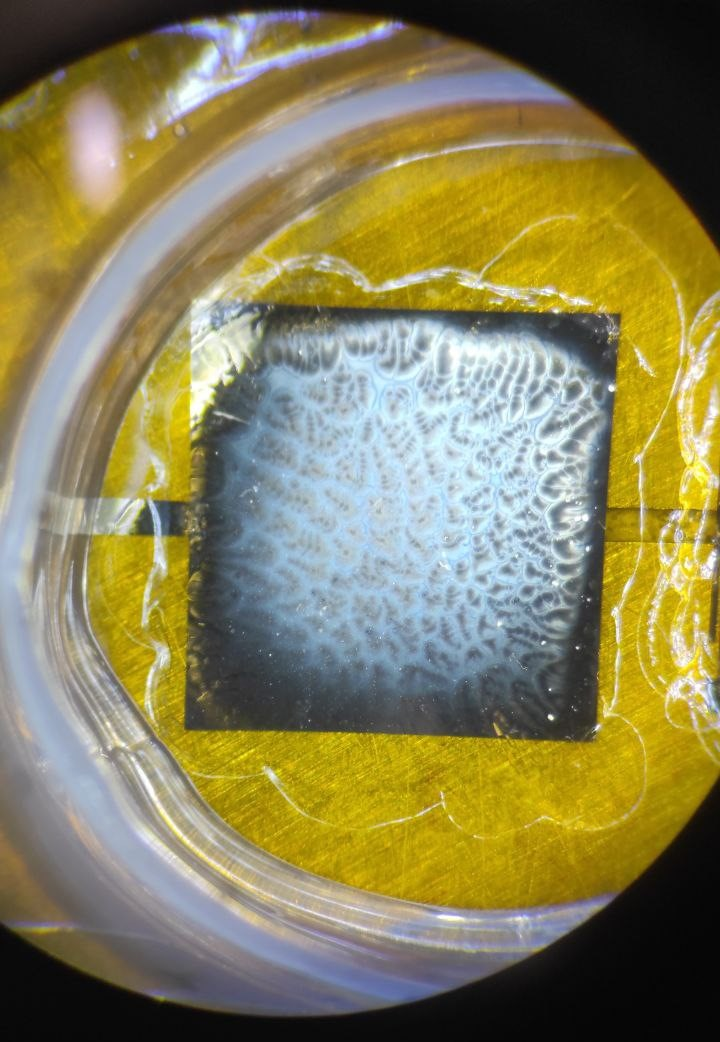
\includegraphics[width=0.3\textwidth]{figures/chapter4/ammonium/gate_membrane.jpg}}
    \caption{Optical image of the ion-sensitive membrane deposited on the gate electrode.}
    \label{fig:ammoniumMembrane}
\end{figure}

In the previous section I demonstrated that I fabricated a stable EG-CNTFET transducer that I can use for a (bio)sensor, based on the standard EG-FET geometry. In this chapter I am going to illustrate the results of a sensor built with such technology.

As a result of the previous work, the functionalization of the CNTs is off-limits, and it remains possible to functionalize the gate. This opens up many possibilities for functionalization, as explained in the introductory section, especially in terms of covalent and stable functionalization that does not interfere with the mobility of the semiconductor. With this in mind, the gate was first functionalized with an ion-selective membrane containing nonactin, as described in section \ref{sec:materials}, which is sensitive to ammonium ions. This membrane is also PVC-based, like the lipophilic membrane on the channel, but it dries differently, resulting in translucency and opacification of the underlying gate, as can be seen in Figure \ref{fig:ammoniumMembrane}.

Once deposited and allowed to dry in an overnight refrigerated environment, the membrane had to have been conditioned 24 hours in 1X PBS containing \SI{1}{mM} ammonium; the reason for the conditioning is not entirely clear; it can be speculated that priming of the ionophore plays an important role, together with the absorption of water molecules, primary and interfering ions \citep{petrelliMethod2023}. \citet{petrelliMethod2023} showed that without this step the sensitivity of the sensor decreases significantly and therefore it is advisable to perform this step.
After conditioning, electrical characterization was performed by first collecting transfer characteristics. The device was allowed to stabilize in 1X PBS for 60 min, after which 5 injections of increasing concentrations of ammonium from 0.01 to 100mM were made, one every 10 min. At the end of the collection, the \ion{} was extracted, with the result shown in Figure \ref{fig:normTransferAmm}. For each injection, the current of the last 4 points was averaged, the standard deviation was calculated, and the result can be seen in Figure \ref{fig:calTransferAmm}. It can be seen that for this type of experiment, the measurements obtained in this way led to an illegible result, in which a difference in current between the first 4 injections is hardly visible and the last one even results at a much lower current, contrary to expectation.

\begin{figure}[]
    \centering
    \subfloat[$\mathrm{I_{ON}^*}$]{%
        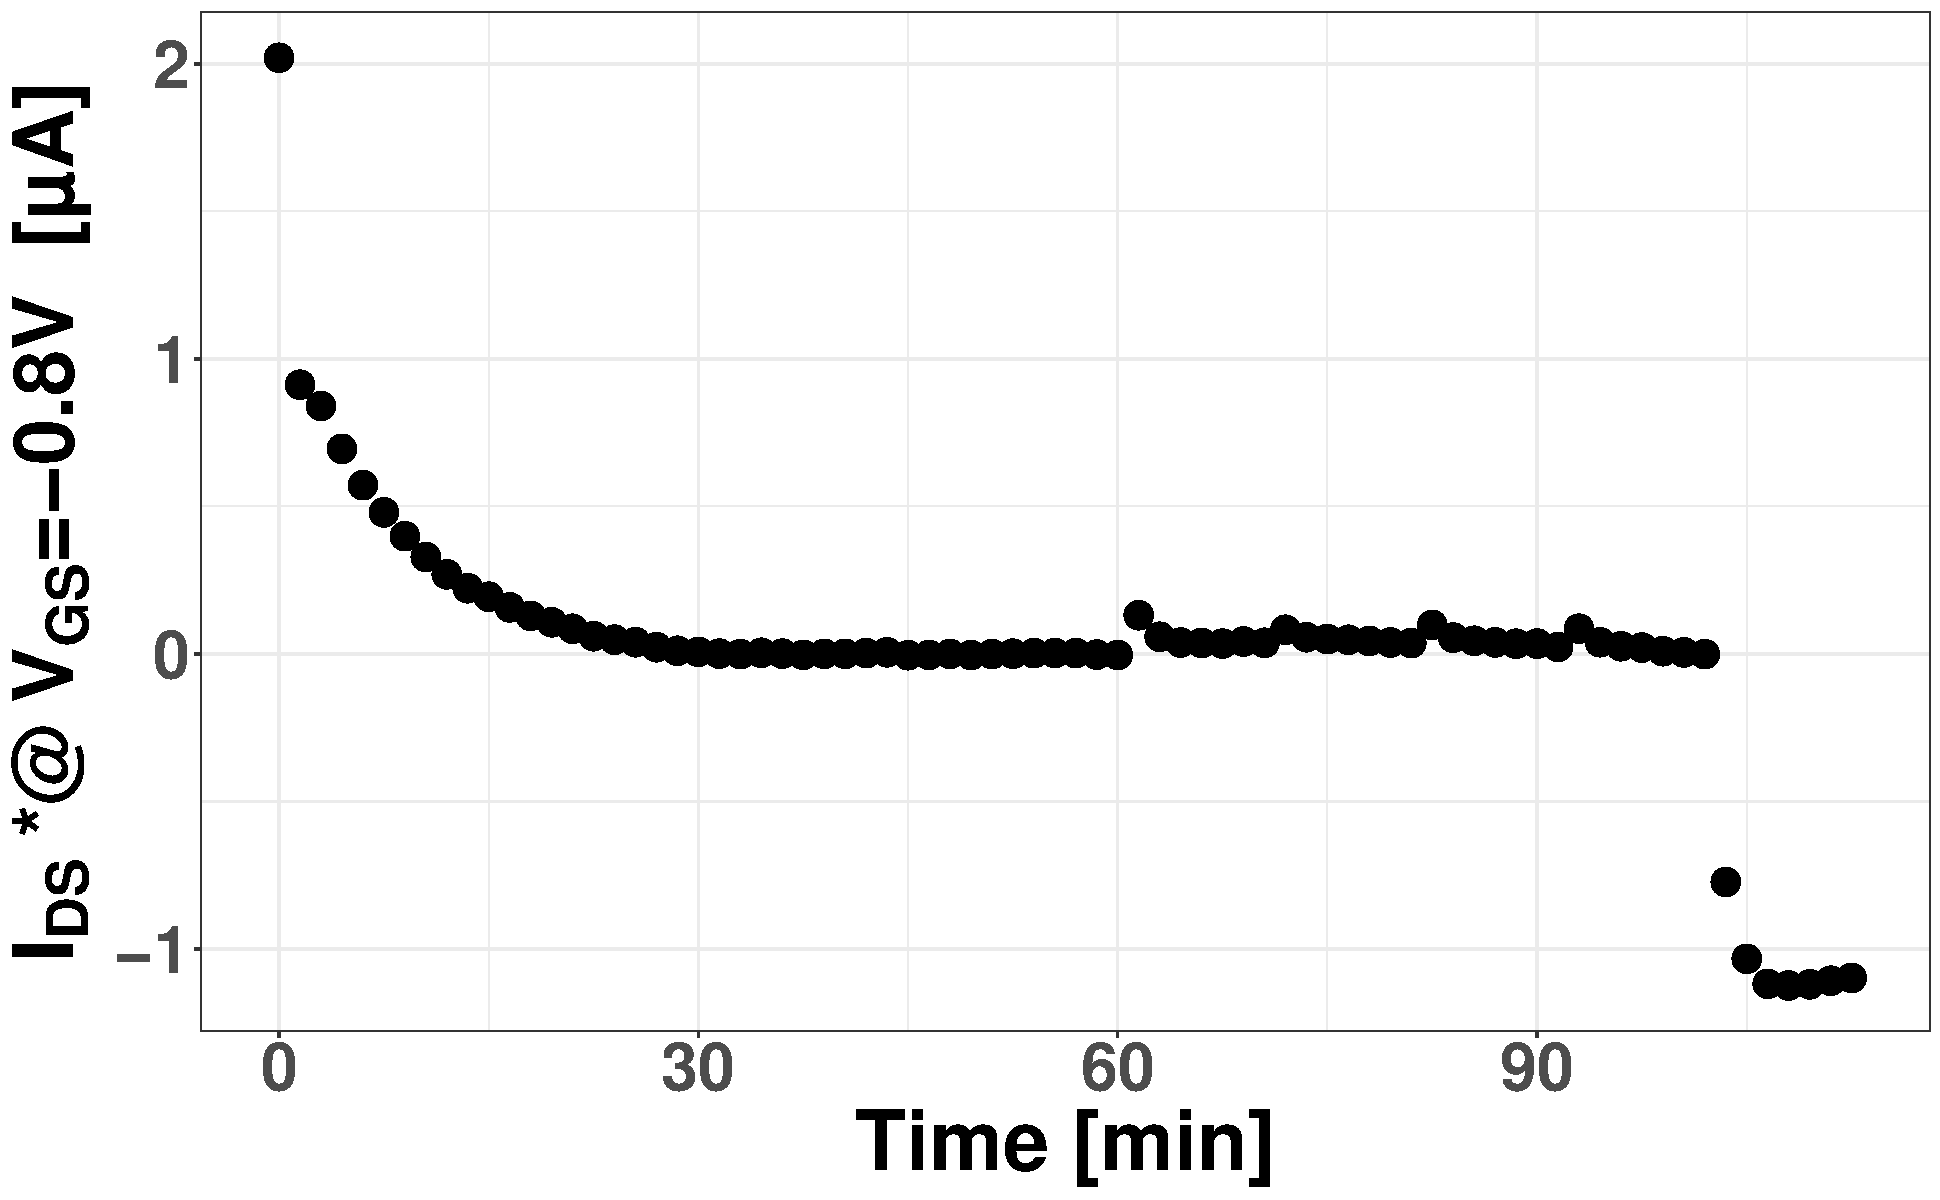
\includegraphics[width=0.45\textwidth]{figures/chapter4/ammonium/correctedPlot_transfers.pdf}
        \label{fig:normTransferAmm}
    }
    \hfill
    \subfloat[Calibration plot]{%
        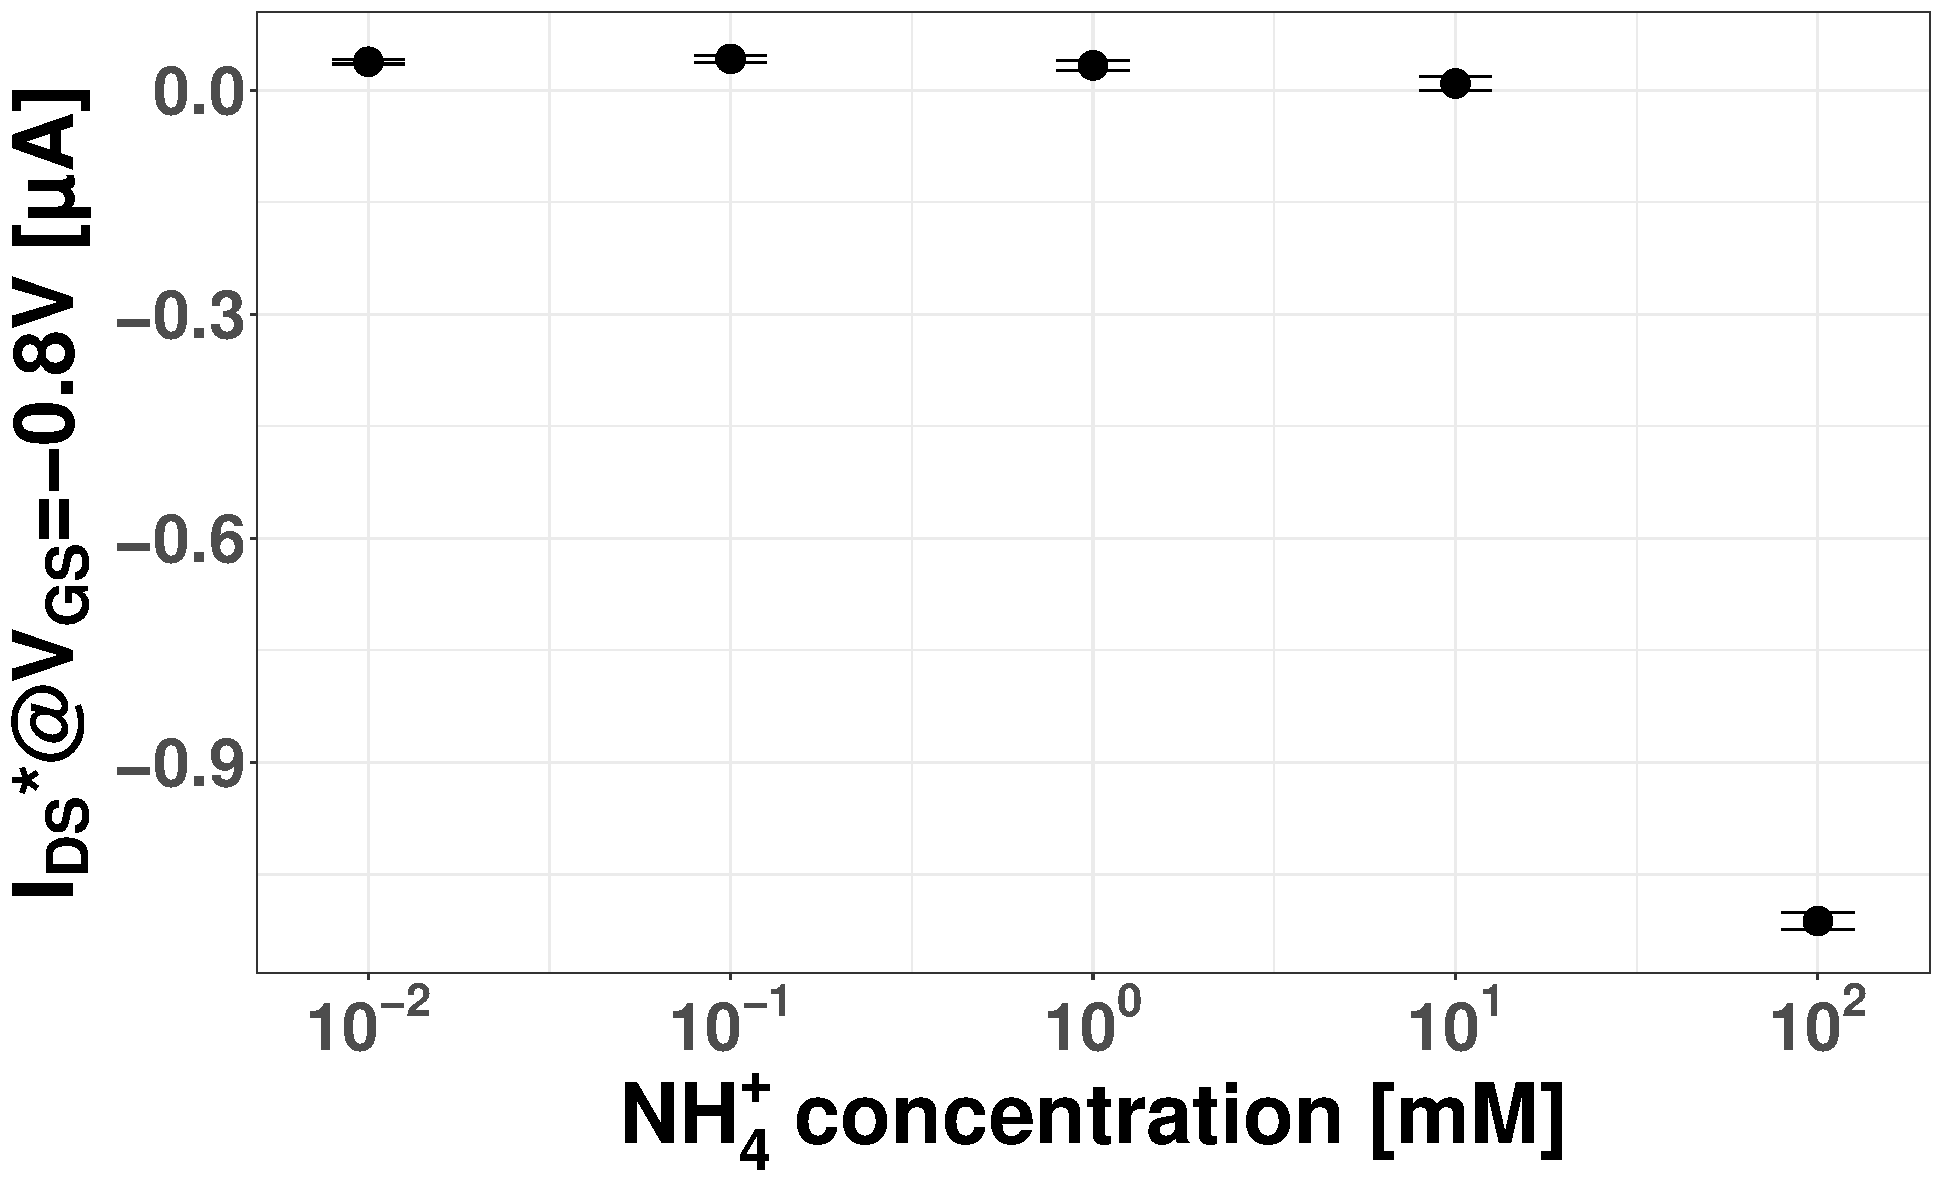
\includegraphics[width=0.45\textwidth]{figures/chapter4/ammonium/calibrationPlot_transfers.pdf}
        \label{fig:calTransferAmm}
    }
    \caption{Electrical characterization of the biosensor: 40 transfer characteristics were collected over the span of \SI{60}{\min} to let the devices stabilize; after this time, 5 increasing concentrations of \amm{} were injected every \SI{10}{\min} (7 transfer curves). The \ion{} was extracted for each curve, the linear fitting calculated over the last 30 minutes of stabilization and the baseline removed, as to obtain the corrected ON current ($\mathrm{I_{ON}^*}$).
    (a) \ioncorr{}. The injection moments are visible as small peaks in the signal.
    (b) Calibration curve obtained by averaging the last four data points of the \ioncorr{} for each concentration. The resulting trend does not match expectations, indicating the need for an alternative measurement or analysis strategy.}
    \label{fig:transferAmm}
\end{figure}

Therefore, the strategy was revised and a new protocol was developed: the experiment was conducted with chronoampetrometry measurements, in which both \vds{} and \vgs{} were fixed and the current was measured over time. In Figure \ref{fig:normChronoAmm} it can be seen how the signal of the injections is much more visible and how they drastically affect the system, which then returns to equilibrium; this is demonstrated by the fact that the current (in modulus) increases very rapidly and very violently after each injection, and then drops and returns to the initial intensity. The calibration plot (Figure \ref{fig:calChronoAmm}) was made in this case by calculating the mean and standard deviation of the current measured during the last 5 minutes of each injection. In this it is possible to observe the expected behavior, \ie{} the signal increases linearly in response to increasing concentrations of analyte, with a sensitivity of \SI{0.14}{\uA \per decade} and a coefficient of determination of 0.94. Thus, it is possible to conclude that an ammonium ion sensor was successfully fabricated using a stable EG-CNTFET as the transducer.

\begin{figure}
    \centering
    \subfloat[Normalized current]{
        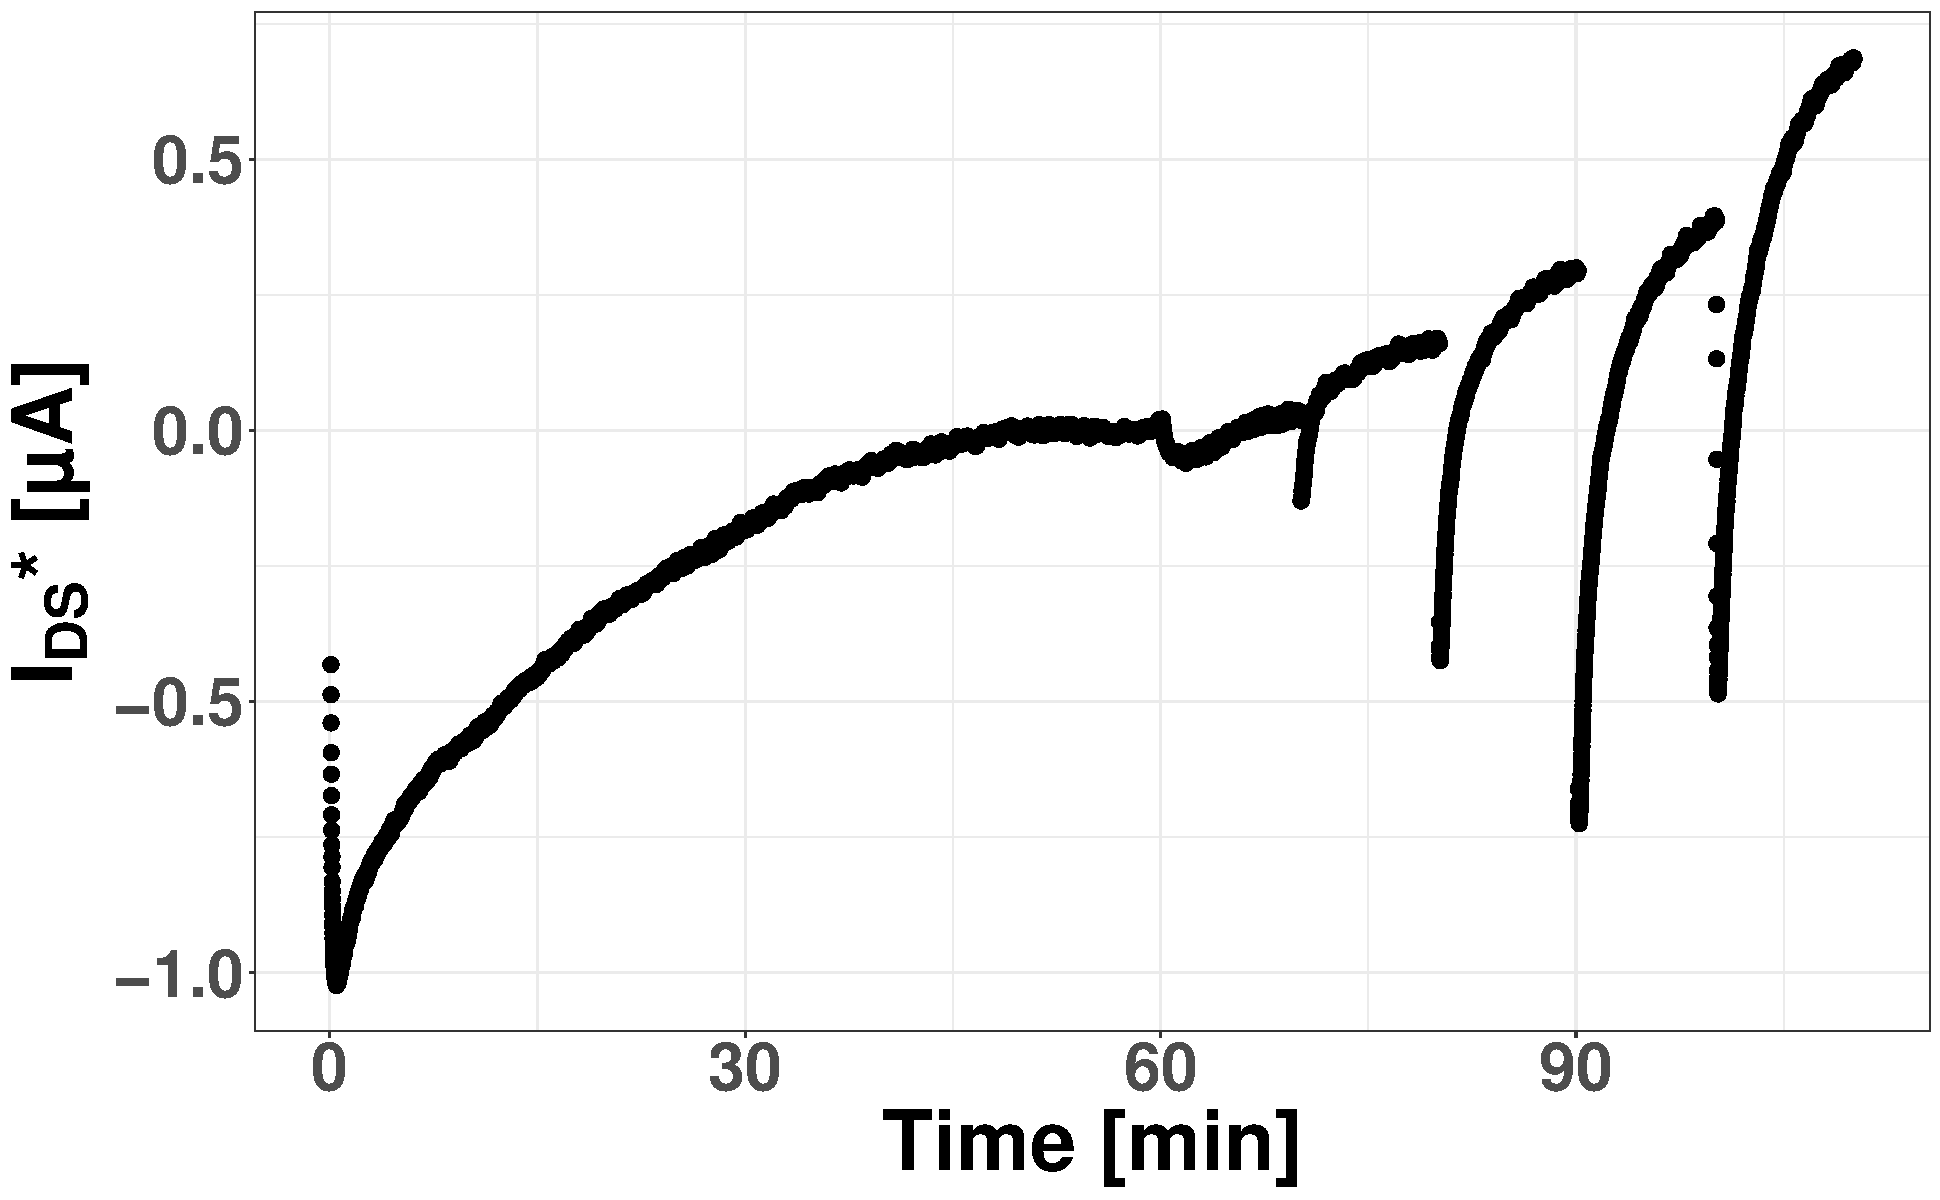
\includegraphics[width=0.45\textwidth]{figures/chapter4/ammonium/correctedPlot-chronoamperometry.pdf}
        \label{fig:normChronoAmm}
    }
    \hfill
    \subfloat[Calibration plot]{
        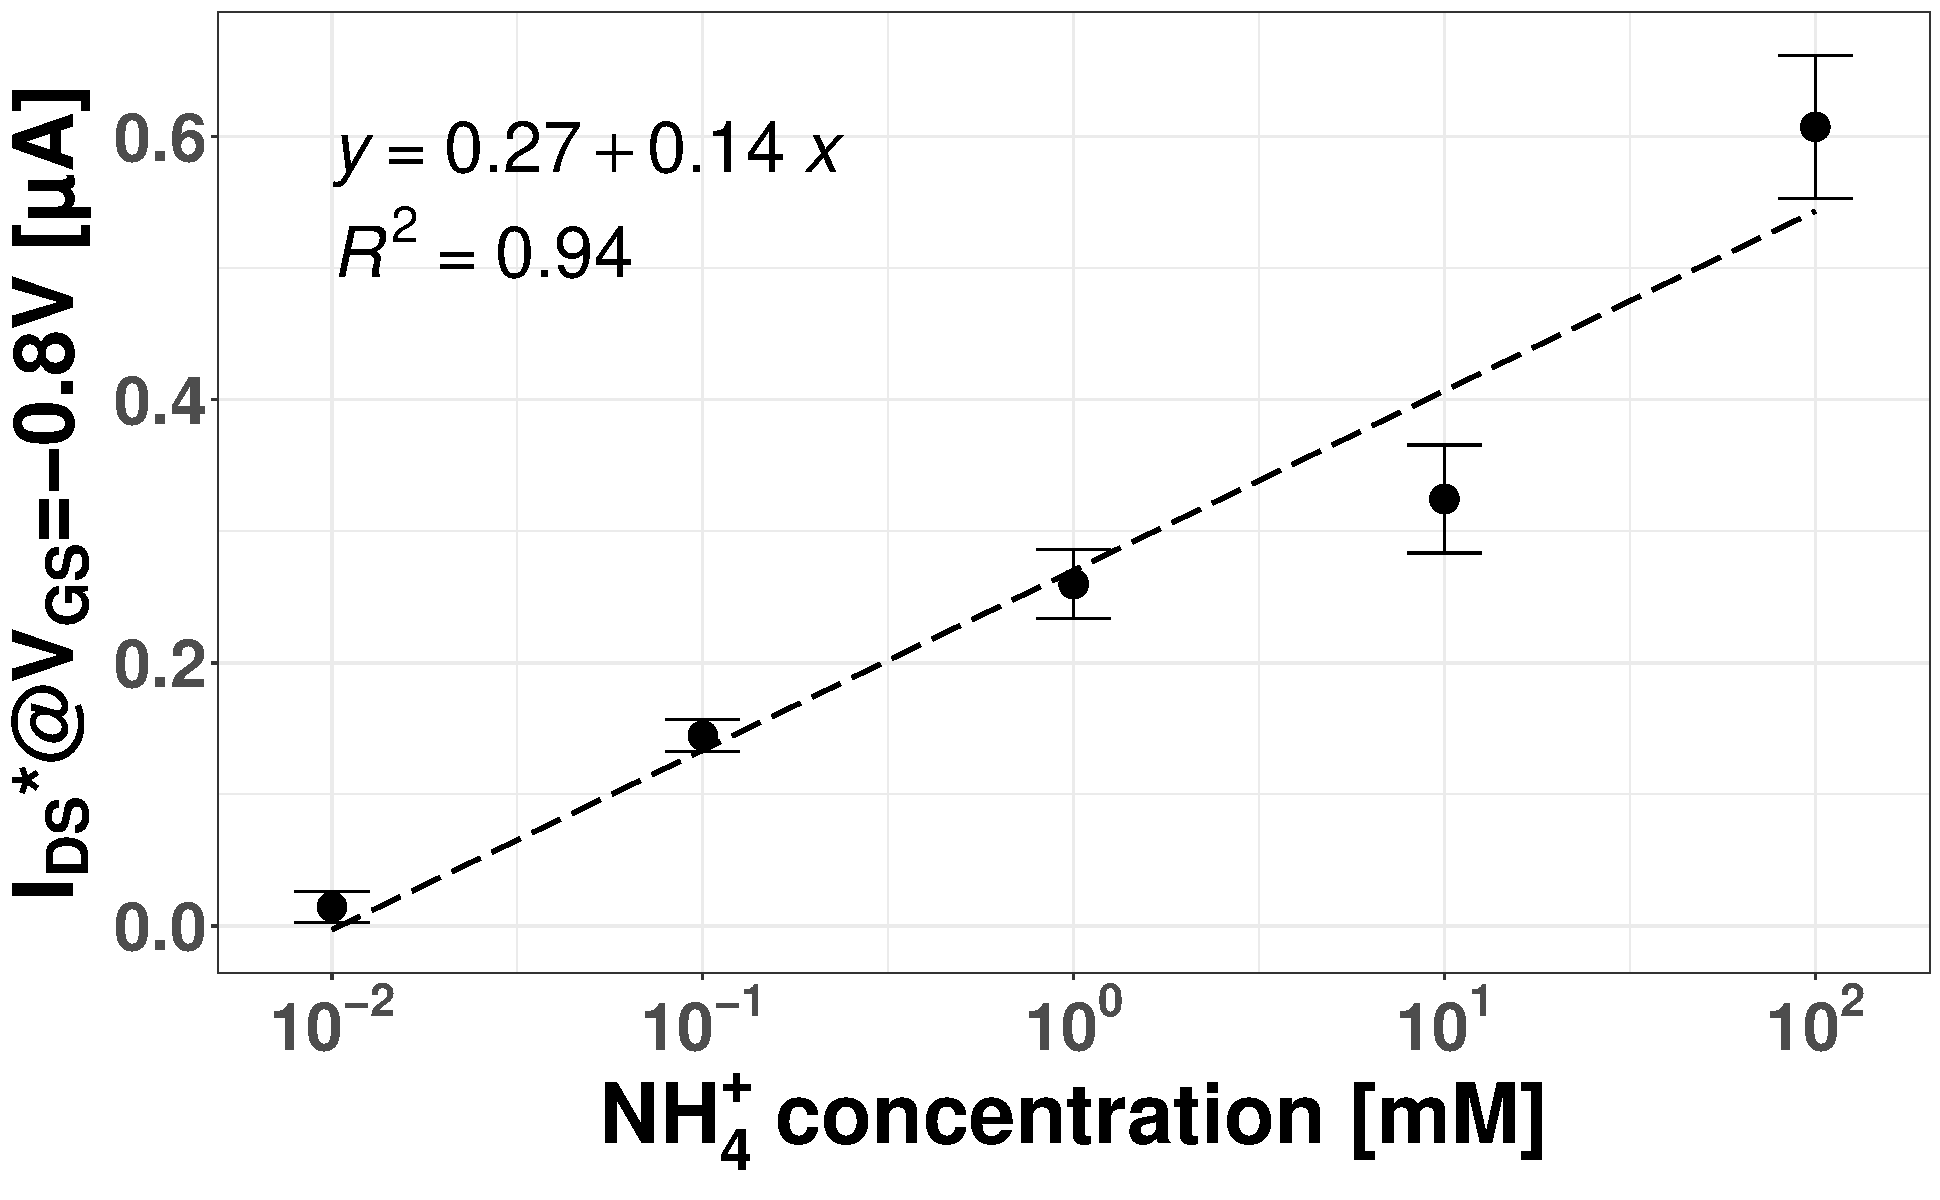
\includegraphics[width=0.45\textwidth]{figures/chapter4/ammonium/calibrationPlot-chronoamperometry.pdf}
        \label{fig:calChronoAmm}
    }
    \caption{Electrical characterization of the biosensor through chronoamperometric measurements: both the \vds{} and \vgs{} and the response of the device was taken over time. The current was fitted with a linear model from \SIrange{30}{60}{\min} and the baseline removed to obtain a corrected current (\idscorr{})
    (a) \idscorr{} over time during chronoamperometric measurements. Injection moments appear as small peaks in the current. 
    (b) Calibration plot obtained by averaging the final four points of the \idscorr{} at each concentration. The linear detection range for \amm{} falls between \SIrange{0.01}{100}{mM}, with a sensitivity of \SI{0.14}{\uA \per decade} and a \rsq{}$= 0.94$.}
    \label{fig:sensing_chronoamperometry}
\end{figure}



%%%%%%%%%%%%%%%%%%%%%%%%%%%%%%%%%%%%%%%%%%%%%%%%%%%%%%%%%%%%%%%%%%%%%%

\section{Histamine detection}
\label{sec:histamine}

\begin{todolist}
    \item what is histamine, why we want to detect it
    \item histamine aptamers
    \item CV
    \item EIS
    \item transfer curves
    \item current vs time
\end{todolist}

\note{To achieve selective detection of histamine using an electrolyte-gated field-effect transistor (EG-FET), the functionalization of the gate electrode is essential. Without a dedicated sensing layer, the device lacks specificity and may respond to various interfering species. This section describes the modification of the gate with a histamine-selective recognition element, enabling precise and reliable detection.}

%%%%%%%%%%%%%%%%%%%%%%%%%%%%%%%%%%%%%%%%%%%%%%%%%%%%%%%%%%%%%%%%%%%%%%

\section{Conclusion}

The stabilized EG-CNTFET platform can be successfully used as a signal transducer in biosensors and is compatible with multiple detection elements. Functionalization with an ion-sensitive membrane resulted in the detection of ammonium in a linear manner ($R^2=0.94$) with a sensitivity of \SI{0.14}{\uA \per decade} at concentrations between \SIrange{0.01}{100}{mM}.
Functionalization with aptamers, on the other hand, detected histamine with a linear trend($R^2=0.95$) in concentrations between \SIrange{0.01}{100}{\micro M}, with a sensitivity of \SI{0.15}{\uA \per decade}.

\newpage
\thispagestyle{empty}
\ % Empty page
\newpage